% Options for packages loaded elsewhere
\PassOptionsToPackage{unicode}{hyperref}
\PassOptionsToPackage{hyphens}{url}
%
\documentclass[
]{article}
\usepackage{amsmath,amssymb}
\usepackage{iftex}
\ifPDFTeX
  \usepackage[T1]{fontenc}
  \usepackage[utf8]{inputenc}
  \usepackage{textcomp} % provide euro and other symbols
\else % if luatex or xetex
  \usepackage{unicode-math} % this also loads fontspec
  \defaultfontfeatures{Scale=MatchLowercase}
  \defaultfontfeatures[\rmfamily]{Ligatures=TeX,Scale=1}
\fi
\usepackage{lmodern}
\ifPDFTeX\else
  % xetex/luatex font selection
\fi
% Use upquote if available, for straight quotes in verbatim environments
\IfFileExists{upquote.sty}{\usepackage{upquote}}{}
\IfFileExists{microtype.sty}{% use microtype if available
  \usepackage[]{microtype}
  \UseMicrotypeSet[protrusion]{basicmath} % disable protrusion for tt fonts
}{}
\makeatletter
\@ifundefined{KOMAClassName}{% if non-KOMA class
  \IfFileExists{parskip.sty}{%
    \usepackage{parskip}
  }{% else
    \setlength{\parindent}{0pt}
    \setlength{\parskip}{6pt plus 2pt minus 1pt}}
}{% if KOMA class
  \KOMAoptions{parskip=half}}
\makeatother
\usepackage{xcolor}
\usepackage[margin=1in]{geometry}
\usepackage{color}
\usepackage{fancyvrb}
\newcommand{\VerbBar}{|}
\newcommand{\VERB}{\Verb[commandchars=\\\{\}]}
\DefineVerbatimEnvironment{Highlighting}{Verbatim}{commandchars=\\\{\}}
% Add ',fontsize=\small' for more characters per line
\usepackage{framed}
\definecolor{shadecolor}{RGB}{248,248,248}
\newenvironment{Shaded}{\begin{snugshade}}{\end{snugshade}}
\newcommand{\AlertTok}[1]{\textcolor[rgb]{0.94,0.16,0.16}{#1}}
\newcommand{\AnnotationTok}[1]{\textcolor[rgb]{0.56,0.35,0.01}{\textbf{\textit{#1}}}}
\newcommand{\AttributeTok}[1]{\textcolor[rgb]{0.13,0.29,0.53}{#1}}
\newcommand{\BaseNTok}[1]{\textcolor[rgb]{0.00,0.00,0.81}{#1}}
\newcommand{\BuiltInTok}[1]{#1}
\newcommand{\CharTok}[1]{\textcolor[rgb]{0.31,0.60,0.02}{#1}}
\newcommand{\CommentTok}[1]{\textcolor[rgb]{0.56,0.35,0.01}{\textit{#1}}}
\newcommand{\CommentVarTok}[1]{\textcolor[rgb]{0.56,0.35,0.01}{\textbf{\textit{#1}}}}
\newcommand{\ConstantTok}[1]{\textcolor[rgb]{0.56,0.35,0.01}{#1}}
\newcommand{\ControlFlowTok}[1]{\textcolor[rgb]{0.13,0.29,0.53}{\textbf{#1}}}
\newcommand{\DataTypeTok}[1]{\textcolor[rgb]{0.13,0.29,0.53}{#1}}
\newcommand{\DecValTok}[1]{\textcolor[rgb]{0.00,0.00,0.81}{#1}}
\newcommand{\DocumentationTok}[1]{\textcolor[rgb]{0.56,0.35,0.01}{\textbf{\textit{#1}}}}
\newcommand{\ErrorTok}[1]{\textcolor[rgb]{0.64,0.00,0.00}{\textbf{#1}}}
\newcommand{\ExtensionTok}[1]{#1}
\newcommand{\FloatTok}[1]{\textcolor[rgb]{0.00,0.00,0.81}{#1}}
\newcommand{\FunctionTok}[1]{\textcolor[rgb]{0.13,0.29,0.53}{\textbf{#1}}}
\newcommand{\ImportTok}[1]{#1}
\newcommand{\InformationTok}[1]{\textcolor[rgb]{0.56,0.35,0.01}{\textbf{\textit{#1}}}}
\newcommand{\KeywordTok}[1]{\textcolor[rgb]{0.13,0.29,0.53}{\textbf{#1}}}
\newcommand{\NormalTok}[1]{#1}
\newcommand{\OperatorTok}[1]{\textcolor[rgb]{0.81,0.36,0.00}{\textbf{#1}}}
\newcommand{\OtherTok}[1]{\textcolor[rgb]{0.56,0.35,0.01}{#1}}
\newcommand{\PreprocessorTok}[1]{\textcolor[rgb]{0.56,0.35,0.01}{\textit{#1}}}
\newcommand{\RegionMarkerTok}[1]{#1}
\newcommand{\SpecialCharTok}[1]{\textcolor[rgb]{0.81,0.36,0.00}{\textbf{#1}}}
\newcommand{\SpecialStringTok}[1]{\textcolor[rgb]{0.31,0.60,0.02}{#1}}
\newcommand{\StringTok}[1]{\textcolor[rgb]{0.31,0.60,0.02}{#1}}
\newcommand{\VariableTok}[1]{\textcolor[rgb]{0.00,0.00,0.00}{#1}}
\newcommand{\VerbatimStringTok}[1]{\textcolor[rgb]{0.31,0.60,0.02}{#1}}
\newcommand{\WarningTok}[1]{\textcolor[rgb]{0.56,0.35,0.01}{\textbf{\textit{#1}}}}
\usepackage{graphicx}
\makeatletter
\def\maxwidth{\ifdim\Gin@nat@width>\linewidth\linewidth\else\Gin@nat@width\fi}
\def\maxheight{\ifdim\Gin@nat@height>\textheight\textheight\else\Gin@nat@height\fi}
\makeatother
% Scale images if necessary, so that they will not overflow the page
% margins by default, and it is still possible to overwrite the defaults
% using explicit options in \includegraphics[width, height, ...]{}
\setkeys{Gin}{width=\maxwidth,height=\maxheight,keepaspectratio}
% Set default figure placement to htbp
\makeatletter
\def\fps@figure{htbp}
\makeatother
\setlength{\emergencystretch}{3em} % prevent overfull lines
\providecommand{\tightlist}{%
  \setlength{\itemsep}{0pt}\setlength{\parskip}{0pt}}
\setcounter{secnumdepth}{-\maxdimen} % remove section numbering
\ifLuaTeX
  \usepackage{selnolig}  % disable illegal ligatures
\fi
\usepackage{bookmark}
\IfFileExists{xurl.sty}{\usepackage{xurl}}{} % add URL line breaks if available
\urlstyle{same}
\hypersetup{
  pdftitle={Bolivia Pilcomayo Heavy Metals Study - Enhanced Visualization},
  pdfauthor={Katerina Bischel},
  hidelinks,
  pdfcreator={LaTeX via pandoc}}

\title{Bolivia Pilcomayo Heavy Metals Study - Enhanced Visualization}
\author{Katerina Bischel}
\date{2025-07-03}

\begin{document}
\maketitle

{
\setcounter{tocdepth}{2}
\tableofcontents
}
\section{Introduction}\label{introduction}

This document analyzes heavy metals contamination in the Pilcomayo River
basin in Bolivia, using data collected in 2006. The analysis compares
contamination levels across water, soil, sediment, vegetation, fish,
human, and animal samples against WHO, Codex Alimentarius, CDC, and
Bolivian reference standards.

\textbf{Key Standards Used:} - WHO Guidelines for Drinking-water Quality
(2017) - Codex Alimentarius Standard 193-1995 Rev.~2018\\
- CDC Lead Reference Value (2021)

\begin{center}\rule{0.5\linewidth}{0.5pt}\end{center}

\section{Water Quality Analysis}\label{water-quality-analysis}

\begin{Shaded}
\begin{Highlighting}[]
\CommentTok{\# Load water data}
\NormalTok{water }\OtherTok{\textless{}{-}} \FunctionTok{read\_csv}\NormalTok{(}\StringTok{"data/ITA\_water\_2006.csv"}\NormalTok{)}
\end{Highlighting}
\end{Shaded}

\subsection{Lead Contamination in Water
Sources}\label{lead-contamination-in-water-sources}

\begin{Shaded}
\begin{Highlighting}[]
\CommentTok{\# WHO standard for lead in drinking water}
\NormalTok{who\_lead\_limit }\OtherTok{\textless{}{-}} \FloatTok{0.01}

\NormalTok{water\_lead\_plot }\OtherTok{\textless{}{-}}\NormalTok{ water }\SpecialCharTok{\%\textgreater{}\%}
  \FunctionTok{mutate}\NormalTok{(}
    \AttributeTok{Location =} \FunctionTok{str\_wrap}\NormalTok{(Location, }\DecValTok{20}\NormalTok{),}
    \AttributeTok{exceeds\_limit =} \StringTok{\textasciigrave{}}\AttributeTok{Pb (mg/l)}\StringTok{\textasciigrave{}} \SpecialCharTok{\textgreater{}}\NormalTok{ who\_lead\_limit,}
    \AttributeTok{risk\_level =} \FunctionTok{case\_when}\NormalTok{(}
      \StringTok{\textasciigrave{}}\AttributeTok{Pb (mg/l)}\StringTok{\textasciigrave{}} \SpecialCharTok{\textless{}=}\NormalTok{ who\_lead\_limit }\SpecialCharTok{\textasciitilde{}} \StringTok{"Safe"}\NormalTok{,}
      \StringTok{\textasciigrave{}}\AttributeTok{Pb (mg/l)}\StringTok{\textasciigrave{}} \SpecialCharTok{\textless{}=}\NormalTok{ who\_lead\_limit }\SpecialCharTok{*} \DecValTok{2} \SpecialCharTok{\textasciitilde{}} \StringTok{"Moderate Risk"}\NormalTok{,}
      \StringTok{\textasciigrave{}}\AttributeTok{Pb (mg/l)}\StringTok{\textasciigrave{}} \SpecialCharTok{\textless{}=}\NormalTok{ who\_lead\_limit }\SpecialCharTok{*} \DecValTok{5} \SpecialCharTok{\textasciitilde{}} \StringTok{"High Risk"}\NormalTok{,}
      \ConstantTok{TRUE} \SpecialCharTok{\textasciitilde{}} \StringTok{"Critical Risk"}
\NormalTok{    )}
\NormalTok{  ) }\SpecialCharTok{\%\textgreater{}\%}
  \FunctionTok{ggplot}\NormalTok{(}\FunctionTok{aes}\NormalTok{(}\AttributeTok{x =} \FunctionTok{reorder}\NormalTok{(Location, }\StringTok{\textasciigrave{}}\AttributeTok{Pb (mg/l)}\StringTok{\textasciigrave{}}\NormalTok{), }\AttributeTok{y =} \StringTok{\textasciigrave{}}\AttributeTok{Pb (mg/l)}\StringTok{\textasciigrave{}}\NormalTok{, }\AttributeTok{fill =}\NormalTok{ risk\_level)) }\SpecialCharTok{+}
  \FunctionTok{geom\_col}\NormalTok{(}\AttributeTok{alpha =} \FloatTok{0.8}\NormalTok{, }\AttributeTok{width =} \FloatTok{0.7}\NormalTok{) }\SpecialCharTok{+}
  \FunctionTok{geom\_hline}\NormalTok{(}
    \AttributeTok{yintercept =}\NormalTok{ who\_lead\_limit, }
    \AttributeTok{color =}\NormalTok{ colors\_danger, }
    \AttributeTok{linetype =} \StringTok{"dashed"}\NormalTok{, }
    \AttributeTok{size =} \FloatTok{1.2}\NormalTok{,}
    \AttributeTok{alpha =} \FloatTok{0.8}
\NormalTok{  ) }\SpecialCharTok{+}
  \FunctionTok{annotate}\NormalTok{(}
    \StringTok{"text"}\NormalTok{,}
    \AttributeTok{x =} \DecValTok{3}\NormalTok{, }\AttributeTok{y =}\NormalTok{ who\_lead\_limit }\SpecialCharTok{+} \FloatTok{0.05}\NormalTok{,}
    \AttributeTok{label =} \StringTok{"WHO Limit (0.01 mg/L)"}\NormalTok{,}
    \AttributeTok{color =}\NormalTok{ colors\_danger,}
    \AttributeTok{size =} \DecValTok{4}\NormalTok{,}
    \AttributeTok{fontface =} \StringTok{"bold"}
\NormalTok{  ) }\SpecialCharTok{+}
  \FunctionTok{scale\_fill\_manual}\NormalTok{(}
    \AttributeTok{values =} \FunctionTok{c}\NormalTok{(}\StringTok{"Safe"} \OtherTok{=}\NormalTok{ colors\_safe, }
               \StringTok{"Moderate Risk"} \OtherTok{=}\NormalTok{ colors\_warning, }
               \StringTok{"High Risk"} \OtherTok{=} \StringTok{"\#e67e22"}\NormalTok{, }
               \StringTok{"Critical Risk"} \OtherTok{=}\NormalTok{ colors\_danger),}
    \AttributeTok{name =} \StringTok{"Risk Level"}
\NormalTok{  ) }\SpecialCharTok{+}
  \FunctionTok{scale\_y\_continuous}\NormalTok{(}
    \AttributeTok{labels =}\NormalTok{ scales}\SpecialCharTok{::}\FunctionTok{number\_format}\NormalTok{(}\AttributeTok{accuracy =} \FloatTok{0.01}\NormalTok{),}
    \AttributeTok{expand =} \FunctionTok{expansion}\NormalTok{(}\AttributeTok{mult =} \FunctionTok{c}\NormalTok{(}\DecValTok{0}\NormalTok{, }\FloatTok{0.1}\NormalTok{))}
\NormalTok{  ) }\SpecialCharTok{+}
  \FunctionTok{labs}\NormalTok{(}
    \AttributeTok{title =} \StringTok{"**Lead Contamination in Water Sources**"}\NormalTok{,}
    \AttributeTok{subtitle =} \StringTok{"Comparison with WHO drinking water guidelines | Higher values indicate greater contamination risk"}\NormalTok{,}
    \AttributeTok{x =} \StringTok{"Sampling Location"}\NormalTok{,}
    \AttributeTok{y =} \StringTok{"Lead Concentration (mg/L)"}\NormalTok{,}
    \AttributeTok{caption =} \StringTok{"Data: Bolivia Pilcomayo River Basin Study 2006 | WHO Standard: 0.01 mg/L"}
\NormalTok{  ) }\SpecialCharTok{+}
  \FunctionTok{theme\_enhanced}\NormalTok{() }\SpecialCharTok{+}
  \FunctionTok{coord\_flip}\NormalTok{()}

\NormalTok{water\_lead\_plot}
\end{Highlighting}
\end{Shaded}

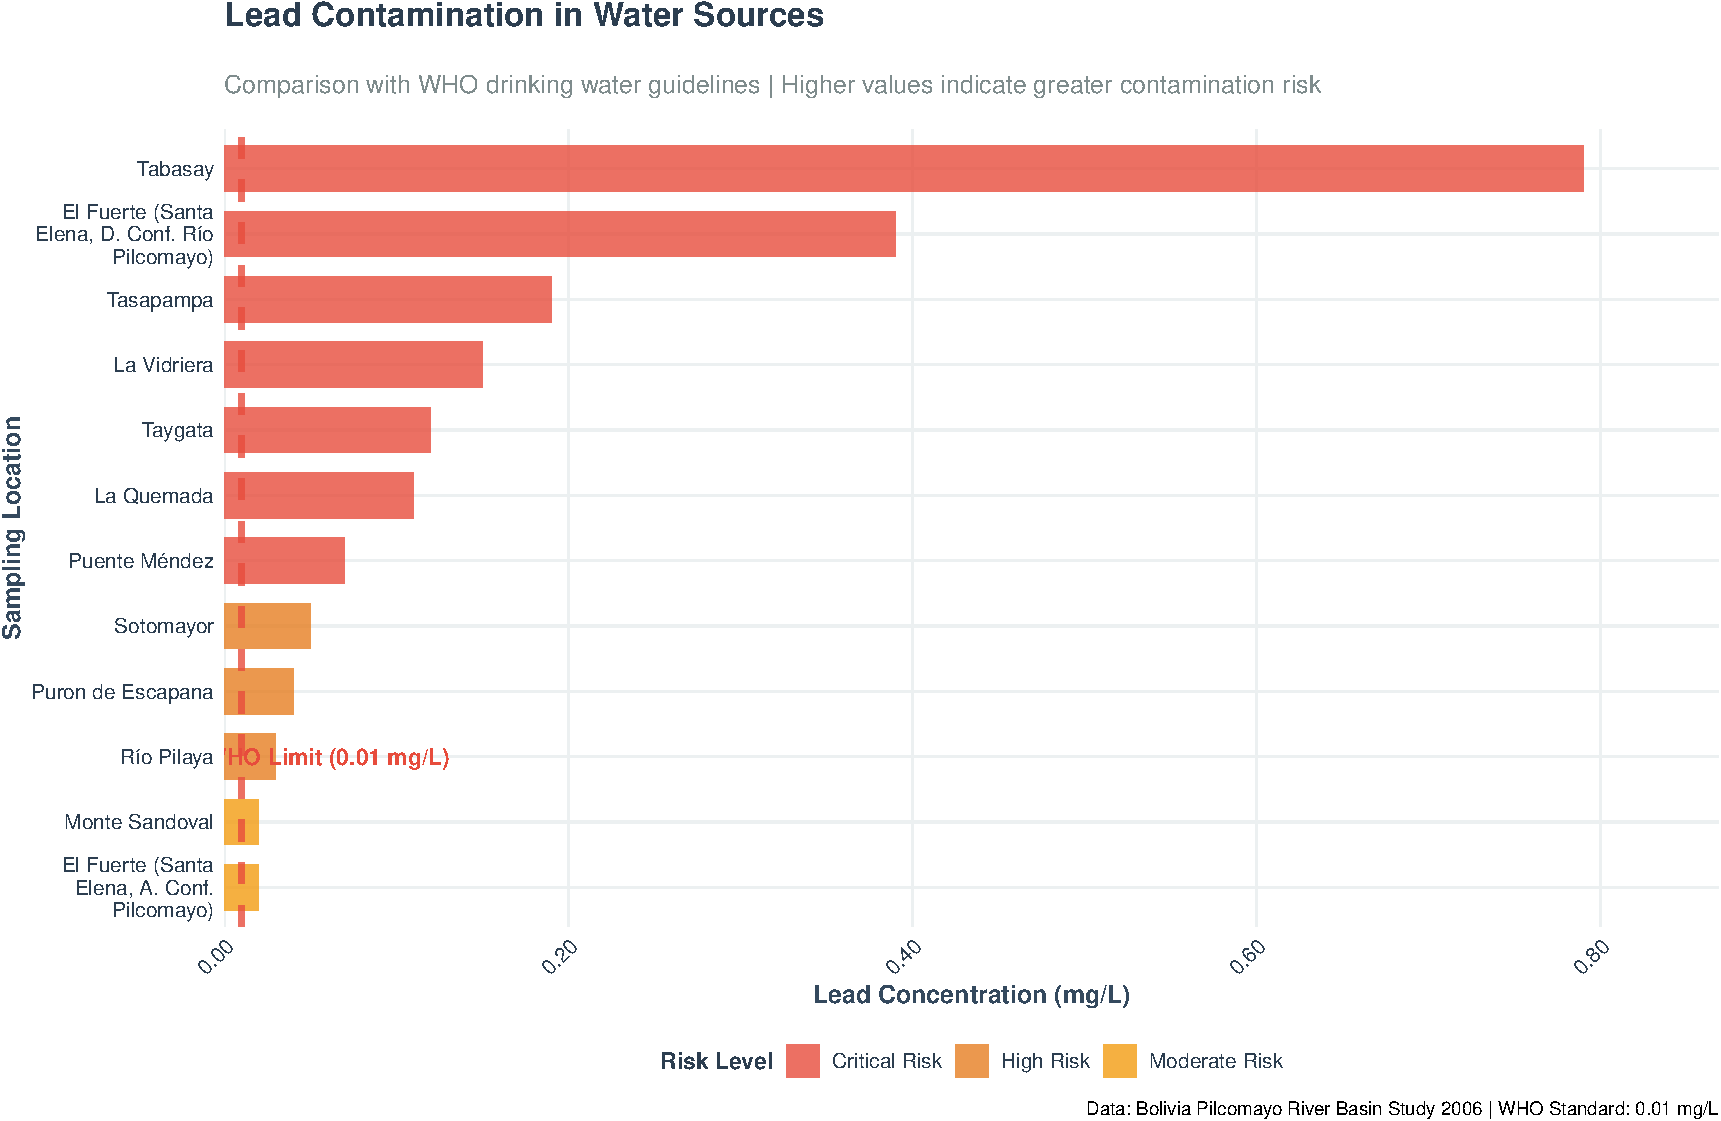
\includegraphics{WHO_standards_pdf_02_files/figure-latex/lead-water-1.pdf}

\subsection{Mercury Contamination in Water
Sources}\label{mercury-contamination-in-water-sources}

\begin{Shaded}
\begin{Highlighting}[]
\CommentTok{\# WHO standard for mercury in drinking water}
\NormalTok{who\_mercury\_limit }\OtherTok{\textless{}{-}} \FloatTok{0.006}

\NormalTok{water\_mercury\_plot }\OtherTok{\textless{}{-}}\NormalTok{ water }\SpecialCharTok{\%\textgreater{}\%}
  \FunctionTok{mutate}\NormalTok{(}
    \AttributeTok{Location =} \FunctionTok{str\_wrap}\NormalTok{(Location, }\DecValTok{20}\NormalTok{),}
    \AttributeTok{exceeds\_limit =} \StringTok{\textasciigrave{}}\AttributeTok{Hg (mg/l)}\StringTok{\textasciigrave{}} \SpecialCharTok{\textgreater{}}\NormalTok{ who\_mercury\_limit,}
    \AttributeTok{risk\_level =} \FunctionTok{case\_when}\NormalTok{(}
      \StringTok{\textasciigrave{}}\AttributeTok{Hg (mg/l)}\StringTok{\textasciigrave{}} \SpecialCharTok{\textless{}=}\NormalTok{ who\_mercury\_limit }\SpecialCharTok{\textasciitilde{}} \StringTok{"Safe"}\NormalTok{,}
      \StringTok{\textasciigrave{}}\AttributeTok{Hg (mg/l)}\StringTok{\textasciigrave{}} \SpecialCharTok{\textless{}=}\NormalTok{ who\_mercury\_limit }\SpecialCharTok{*} \FloatTok{1.5} \SpecialCharTok{\textasciitilde{}} \StringTok{"Moderate Risk"}\NormalTok{,}
      \ConstantTok{TRUE} \SpecialCharTok{\textasciitilde{}} \StringTok{"High Risk"}
\NormalTok{    )}
\NormalTok{  ) }\SpecialCharTok{\%\textgreater{}\%}
  \FunctionTok{ggplot}\NormalTok{(}\FunctionTok{aes}\NormalTok{(}\AttributeTok{x =} \FunctionTok{reorder}\NormalTok{(Location, }\StringTok{\textasciigrave{}}\AttributeTok{Hg (mg/l)}\StringTok{\textasciigrave{}}\NormalTok{), }\AttributeTok{y =} \StringTok{\textasciigrave{}}\AttributeTok{Hg (mg/l)}\StringTok{\textasciigrave{}}\NormalTok{, }\AttributeTok{fill =}\NormalTok{ risk\_level)) }\SpecialCharTok{+}
  \FunctionTok{geom\_col}\NormalTok{(}\AttributeTok{alpha =} \FloatTok{0.8}\NormalTok{, }\AttributeTok{width =} \FloatTok{0.7}\NormalTok{) }\SpecialCharTok{+}
  \FunctionTok{geom\_hline}\NormalTok{(}
    \AttributeTok{yintercept =}\NormalTok{ who\_mercury\_limit, }
    \AttributeTok{color =}\NormalTok{ colors\_danger, }
    \AttributeTok{linetype =} \StringTok{"dashed"}\NormalTok{, }
    \AttributeTok{size =} \FloatTok{1.2}\NormalTok{,}
    \AttributeTok{alpha =} \FloatTok{0.8}
\NormalTok{  ) }\SpecialCharTok{+}
  \FunctionTok{annotate}\NormalTok{(}
    \StringTok{"text"}\NormalTok{,}
    \AttributeTok{x =} \DecValTok{3}\NormalTok{, }\AttributeTok{y =}\NormalTok{ who\_mercury\_limit }\SpecialCharTok{+} \FloatTok{0.001}\NormalTok{,}
    \AttributeTok{label =} \StringTok{"WHO Limit (0.006 mg/L)"}\NormalTok{,}
    \AttributeTok{color =}\NormalTok{ colors\_danger,}
    \AttributeTok{size =} \DecValTok{4}\NormalTok{,}
    \AttributeTok{fontface =} \StringTok{"bold"}
\NormalTok{  ) }\SpecialCharTok{+}
  \FunctionTok{scale\_fill\_manual}\NormalTok{(}
    \AttributeTok{values =} \FunctionTok{c}\NormalTok{(}\StringTok{"Safe"} \OtherTok{=}\NormalTok{ colors\_safe, }
               \StringTok{"Moderate Risk"} \OtherTok{=}\NormalTok{ colors\_warning, }
               \StringTok{"High Risk"} \OtherTok{=}\NormalTok{ colors\_danger),}
    \AttributeTok{name =} \StringTok{"Risk Level"}
\NormalTok{  ) }\SpecialCharTok{+}
  \FunctionTok{scale\_y\_continuous}\NormalTok{(}
    \AttributeTok{labels =}\NormalTok{ scales}\SpecialCharTok{::}\FunctionTok{number\_format}\NormalTok{(}\AttributeTok{accuracy =} \FloatTok{0.001}\NormalTok{),}
    \AttributeTok{expand =} \FunctionTok{expansion}\NormalTok{(}\AttributeTok{mult =} \FunctionTok{c}\NormalTok{(}\DecValTok{0}\NormalTok{, }\FloatTok{0.1}\NormalTok{))}
\NormalTok{  ) }\SpecialCharTok{+}
  \FunctionTok{labs}\NormalTok{(}
    \AttributeTok{title =} \StringTok{"**Mercury Contamination in Water Sources**"}\NormalTok{,}
    \AttributeTok{subtitle =} \StringTok{"Comparison with WHO drinking water guidelines | All samples within safe limits"}\NormalTok{,}
    \AttributeTok{x =} \StringTok{"Sampling Location"}\NormalTok{,}
    \AttributeTok{y =} \StringTok{"Mercury Concentration (mg/L)"}\NormalTok{,}
    \AttributeTok{caption =} \StringTok{"Data: Bolivia Pilcomayo River Basin Study 2006 | WHO Standard: 0.006 mg/L"}
\NormalTok{  ) }\SpecialCharTok{+}
  \FunctionTok{theme\_enhanced}\NormalTok{() }\SpecialCharTok{+}
  \FunctionTok{coord\_flip}\NormalTok{()}

\NormalTok{water\_mercury\_plot}
\end{Highlighting}
\end{Shaded}

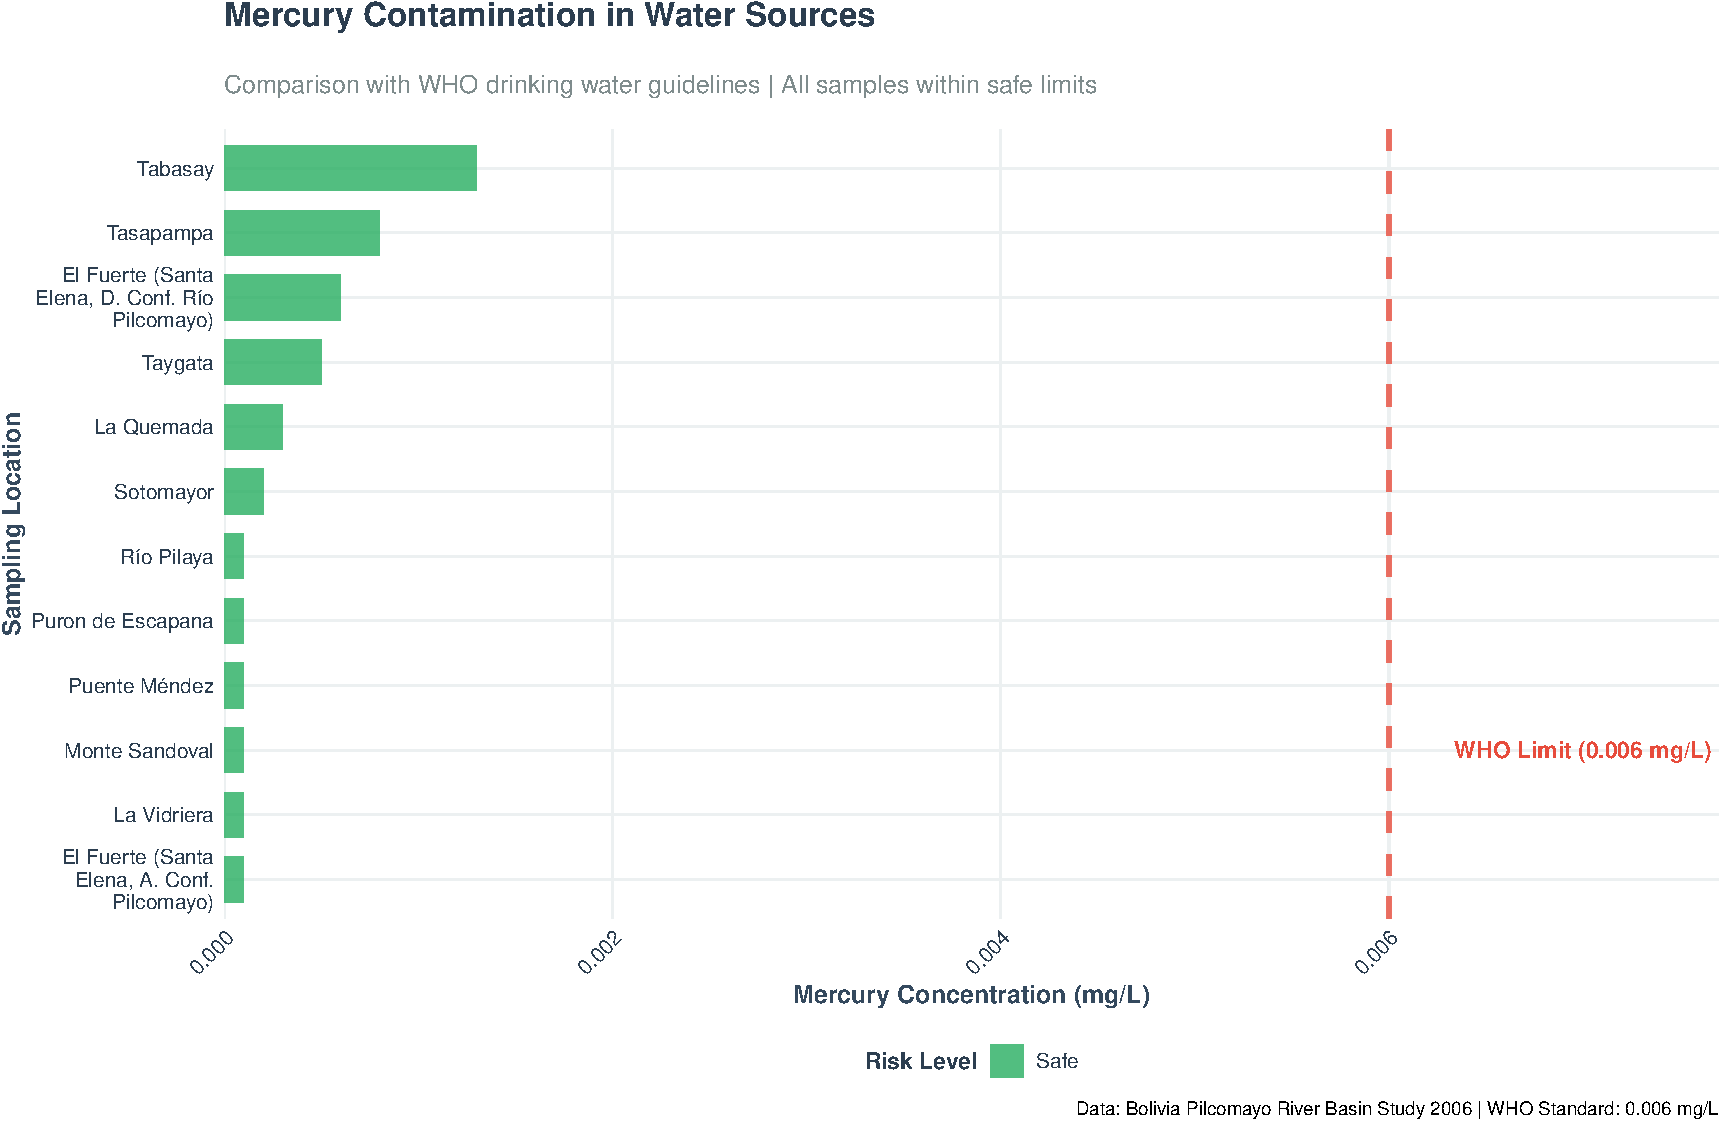
\includegraphics{WHO_standards_pdf_02_files/figure-latex/mercury-water-1.pdf}

\begin{center}\rule{0.5\linewidth}{0.5pt}\end{center}

\section{Soil and Sediment Analysis}\label{soil-and-sediment-analysis}

\begin{Shaded}
\begin{Highlighting}[]
\CommentTok{\# Load soil and sediment data}
\NormalTok{soil }\OtherTok{\textless{}{-}} \FunctionTok{read\_csv}\NormalTok{(}\StringTok{"data/ITA\_soil\_2006.csv"}\NormalTok{)}
\NormalTok{sediment }\OtherTok{\textless{}{-}} \FunctionTok{read\_csv}\NormalTok{(}\StringTok{"data/ITA\_sed\_2006.csv"}\NormalTok{)}

\CommentTok{\# Reference standard for lead in soil}
\NormalTok{soil\_lead\_limit }\OtherTok{\textless{}{-}} \DecValTok{70}
\end{Highlighting}
\end{Shaded}

\subsection{Lead Contamination in
Soil}\label{lead-contamination-in-soil}

\begin{Shaded}
\begin{Highlighting}[]
\NormalTok{soil\_lead\_plot }\OtherTok{\textless{}{-}}\NormalTok{ soil }\SpecialCharTok{\%\textgreater{}\%}
  \FunctionTok{mutate}\NormalTok{(}
    \AttributeTok{Location =} \FunctionTok{str\_wrap}\NormalTok{(Location, }\DecValTok{20}\NormalTok{),}
    \AttributeTok{exceeds\_limit =} \StringTok{\textasciigrave{}}\AttributeTok{Pb (mg/kg)}\StringTok{\textasciigrave{}} \SpecialCharTok{\textgreater{}}\NormalTok{ soil\_lead\_limit,}
    \AttributeTok{risk\_level =} \FunctionTok{case\_when}\NormalTok{(}
      \StringTok{\textasciigrave{}}\AttributeTok{Pb (mg/kg)}\StringTok{\textasciigrave{}} \SpecialCharTok{\textless{}=}\NormalTok{ soil\_lead\_limit }\SpecialCharTok{\textasciitilde{}} \StringTok{"Safe"}\NormalTok{,}
      \StringTok{\textasciigrave{}}\AttributeTok{Pb (mg/kg)}\StringTok{\textasciigrave{}} \SpecialCharTok{\textless{}=}\NormalTok{ soil\_lead\_limit }\SpecialCharTok{*} \DecValTok{3} \SpecialCharTok{\textasciitilde{}} \StringTok{"Moderate Risk"}\NormalTok{,}
      \StringTok{\textasciigrave{}}\AttributeTok{Pb (mg/kg)}\StringTok{\textasciigrave{}} \SpecialCharTok{\textless{}=}\NormalTok{ soil\_lead\_limit }\SpecialCharTok{*} \DecValTok{10} \SpecialCharTok{\textasciitilde{}} \StringTok{"High Risk"}\NormalTok{,}
      \ConstantTok{TRUE} \SpecialCharTok{\textasciitilde{}} \StringTok{"Critical Risk"}
\NormalTok{    )}
\NormalTok{  ) }\SpecialCharTok{\%\textgreater{}\%}
  \FunctionTok{ggplot}\NormalTok{(}\FunctionTok{aes}\NormalTok{(}\AttributeTok{x =} \FunctionTok{reorder}\NormalTok{(Location, }\StringTok{\textasciigrave{}}\AttributeTok{Pb (mg/kg)}\StringTok{\textasciigrave{}}\NormalTok{), }\AttributeTok{y =} \StringTok{\textasciigrave{}}\AttributeTok{Pb (mg/kg)}\StringTok{\textasciigrave{}}\NormalTok{, }\AttributeTok{fill =}\NormalTok{ risk\_level)) }\SpecialCharTok{+}
  \FunctionTok{geom\_col}\NormalTok{(}\AttributeTok{alpha =} \FloatTok{0.8}\NormalTok{, }\AttributeTok{width =} \FloatTok{0.7}\NormalTok{) }\SpecialCharTok{+}
  \FunctionTok{geom\_hline}\NormalTok{(}
    \AttributeTok{yintercept =}\NormalTok{ soil\_lead\_limit, }
    \AttributeTok{color =}\NormalTok{ colors\_danger, }
    \AttributeTok{linetype =} \StringTok{"dashed"}\NormalTok{, }
    \AttributeTok{size =} \FloatTok{1.2}\NormalTok{,}
    \AttributeTok{alpha =} \FloatTok{0.8}
\NormalTok{  ) }\SpecialCharTok{+}
  \FunctionTok{annotate}\NormalTok{(}
    \StringTok{"text"}\NormalTok{,}
    \AttributeTok{x =} \DecValTok{3}\NormalTok{, }\AttributeTok{y =}\NormalTok{ soil\_lead\_limit }\SpecialCharTok{+} \DecValTok{100}\NormalTok{,}
    \AttributeTok{label =} \StringTok{"Reference Limit (70 mg/kg)"}\NormalTok{,}
    \AttributeTok{color =}\NormalTok{ colors\_danger,}
    \AttributeTok{size =} \DecValTok{4}\NormalTok{,}
    \AttributeTok{fontface =} \StringTok{"bold"}
\NormalTok{  ) }\SpecialCharTok{+}
  \FunctionTok{scale\_fill\_manual}\NormalTok{(}
    \AttributeTok{values =} \FunctionTok{c}\NormalTok{(}\StringTok{"Safe"} \OtherTok{=}\NormalTok{ colors\_safe, }
               \StringTok{"Moderate Risk"} \OtherTok{=}\NormalTok{ colors\_warning, }
               \StringTok{"High Risk"} \OtherTok{=} \StringTok{"\#e67e22"}\NormalTok{, }
               \StringTok{"Critical Risk"} \OtherTok{=}\NormalTok{ colors\_danger),}
    \AttributeTok{name =} \StringTok{"Risk Level"}
\NormalTok{  ) }\SpecialCharTok{+}
  \FunctionTok{scale\_y\_continuous}\NormalTok{(}
    \AttributeTok{labels =}\NormalTok{ scales}\SpecialCharTok{::}\FunctionTok{comma\_format}\NormalTok{(),}
    \AttributeTok{expand =} \FunctionTok{expansion}\NormalTok{(}\AttributeTok{mult =} \FunctionTok{c}\NormalTok{(}\DecValTok{0}\NormalTok{, }\FloatTok{0.1}\NormalTok{))}
\NormalTok{  ) }\SpecialCharTok{+}
  \FunctionTok{labs}\NormalTok{(}
    \AttributeTok{title =} \StringTok{"**Lead Contamination in Soil Samples**"}\NormalTok{,}
    \AttributeTok{subtitle =} \StringTok{"Several locations show severe contamination exceeding safe limits"}\NormalTok{,}
    \AttributeTok{x =} \StringTok{"Sampling Location"}\NormalTok{,}
    \AttributeTok{y =} \StringTok{"Lead Concentration (mg/kg)"}\NormalTok{,}
    \AttributeTok{caption =} \StringTok{"Data: Bolivia Pilcomayo River Basin Study 2006 | Reference Standard: 70 mg/kg"}
\NormalTok{  ) }\SpecialCharTok{+}
  \FunctionTok{theme\_enhanced}\NormalTok{() }\SpecialCharTok{+}
  \FunctionTok{coord\_flip}\NormalTok{()}

\NormalTok{soil\_lead\_plot}
\end{Highlighting}
\end{Shaded}

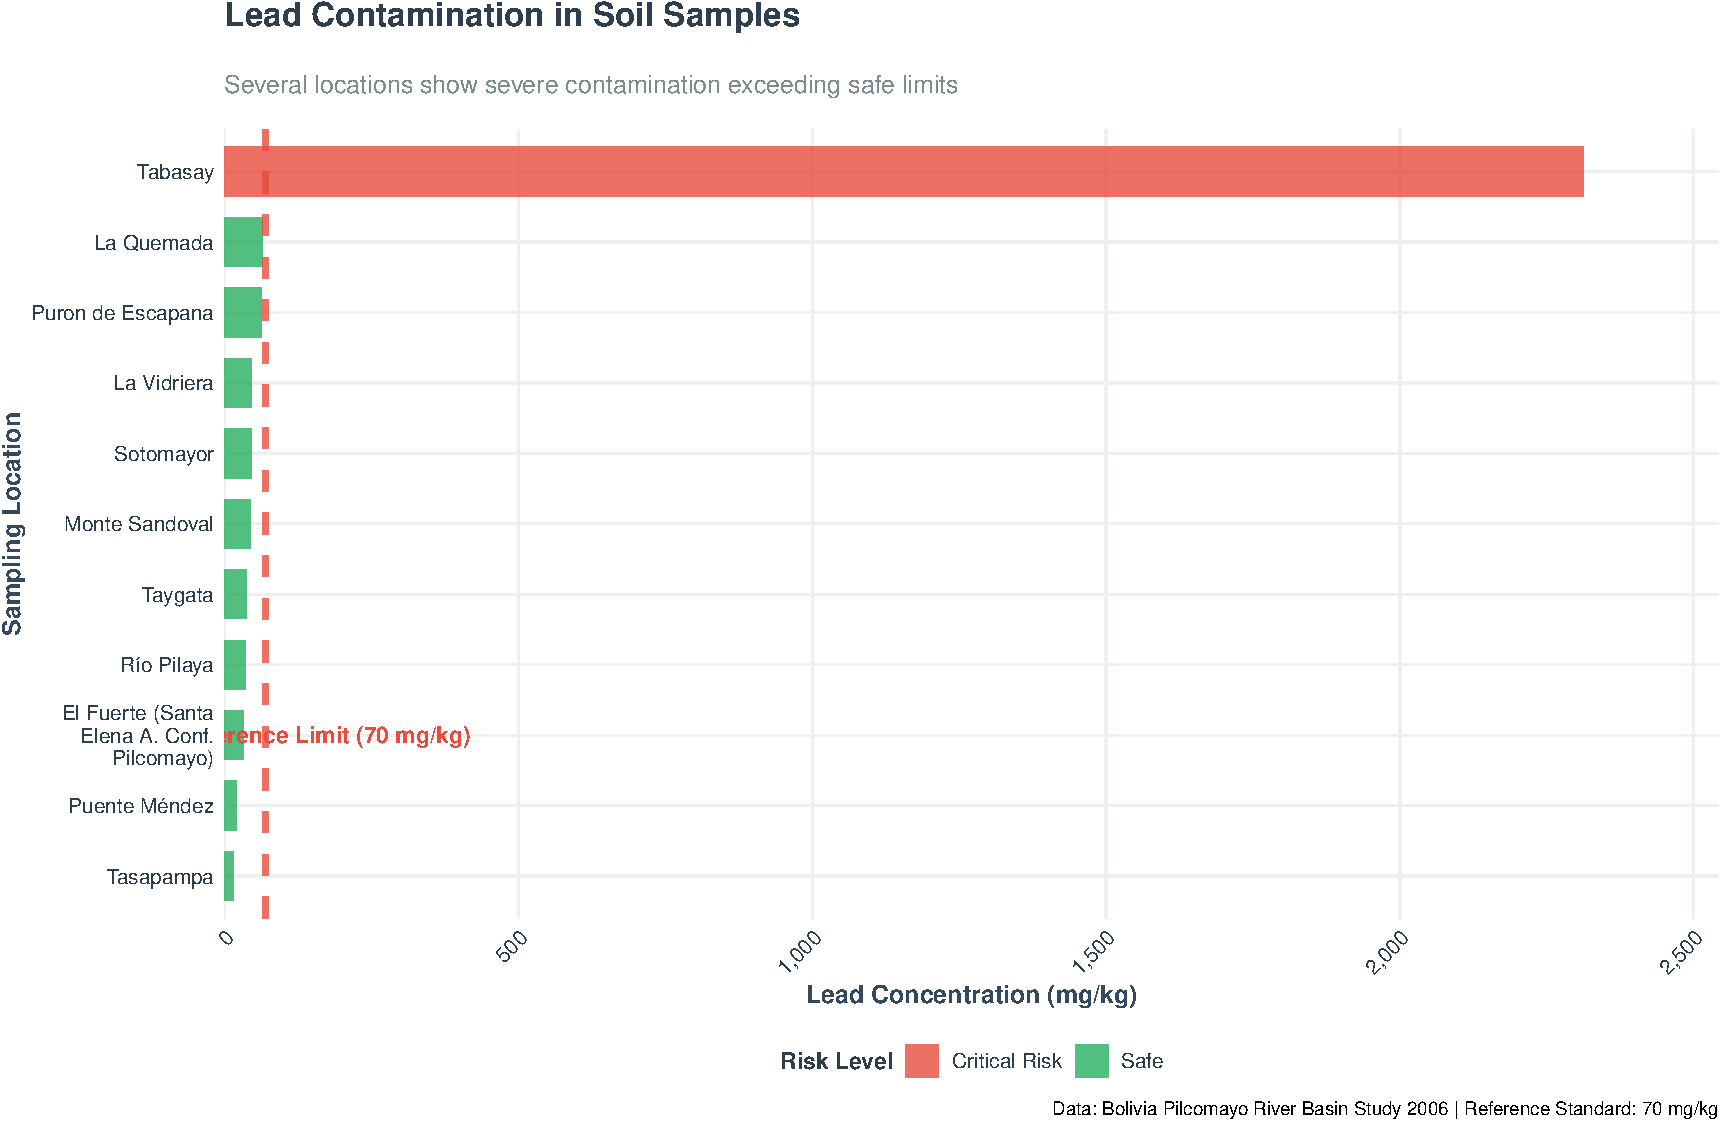
\includegraphics{WHO_standards_pdf_02_files/figure-latex/soil-lead-1.pdf}

\subsection{Lead Contamination in
Sediment}\label{lead-contamination-in-sediment}

\begin{Shaded}
\begin{Highlighting}[]
\NormalTok{sediment\_lead\_plot }\OtherTok{\textless{}{-}}\NormalTok{ sediment }\SpecialCharTok{\%\textgreater{}\%}
  \FunctionTok{mutate}\NormalTok{(}
    \AttributeTok{Location =} \FunctionTok{str\_wrap}\NormalTok{(Location, }\DecValTok{20}\NormalTok{),}
    \AttributeTok{exceeds\_limit =} \StringTok{\textasciigrave{}}\AttributeTok{Pb (mg/kg)}\StringTok{\textasciigrave{}} \SpecialCharTok{\textgreater{}}\NormalTok{ soil\_lead\_limit,}
    \AttributeTok{risk\_level =} \FunctionTok{case\_when}\NormalTok{(}
      \StringTok{\textasciigrave{}}\AttributeTok{Pb (mg/kg)}\StringTok{\textasciigrave{}} \SpecialCharTok{\textless{}=}\NormalTok{ soil\_lead\_limit }\SpecialCharTok{\textasciitilde{}} \StringTok{"Safe"}\NormalTok{,}
      \StringTok{\textasciigrave{}}\AttributeTok{Pb (mg/kg)}\StringTok{\textasciigrave{}} \SpecialCharTok{\textless{}=}\NormalTok{ soil\_lead\_limit }\SpecialCharTok{*} \FloatTok{1.5} \SpecialCharTok{\textasciitilde{}} \StringTok{"Moderate Risk"}\NormalTok{,}
      \ConstantTok{TRUE} \SpecialCharTok{\textasciitilde{}} \StringTok{"High Risk"}
\NormalTok{    )}
\NormalTok{  ) }\SpecialCharTok{\%\textgreater{}\%}
  \FunctionTok{ggplot}\NormalTok{(}\FunctionTok{aes}\NormalTok{(}\AttributeTok{x =} \FunctionTok{reorder}\NormalTok{(Location, }\StringTok{\textasciigrave{}}\AttributeTok{Pb (mg/kg)}\StringTok{\textasciigrave{}}\NormalTok{), }\AttributeTok{y =} \StringTok{\textasciigrave{}}\AttributeTok{Pb (mg/kg)}\StringTok{\textasciigrave{}}\NormalTok{, }\AttributeTok{fill =}\NormalTok{ risk\_level)) }\SpecialCharTok{+}
  \FunctionTok{geom\_col}\NormalTok{(}\AttributeTok{alpha =} \FloatTok{0.8}\NormalTok{, }\AttributeTok{width =} \FloatTok{0.7}\NormalTok{) }\SpecialCharTok{+}
  \FunctionTok{geom\_hline}\NormalTok{(}
    \AttributeTok{yintercept =}\NormalTok{ soil\_lead\_limit, }
    \AttributeTok{color =}\NormalTok{ colors\_danger, }
    \AttributeTok{linetype =} \StringTok{"dashed"}\NormalTok{, }
    \AttributeTok{size =} \FloatTok{1.2}\NormalTok{,}
    \AttributeTok{alpha =} \FloatTok{0.8}
\NormalTok{  ) }\SpecialCharTok{+}
  \FunctionTok{annotate}\NormalTok{(}
    \StringTok{"text"}\NormalTok{,}
    \AttributeTok{x =} \DecValTok{3}\NormalTok{, }\AttributeTok{y =}\NormalTok{ soil\_lead\_limit }\SpecialCharTok{+} \DecValTok{5}\NormalTok{,}
    \AttributeTok{label =} \StringTok{"Reference Limit (70 mg/kg)"}\NormalTok{,}
    \AttributeTok{color =}\NormalTok{ colors\_danger,}
    \AttributeTok{size =} \DecValTok{4}\NormalTok{,}
    \AttributeTok{fontface =} \StringTok{"bold"}
\NormalTok{  ) }\SpecialCharTok{+}
  \FunctionTok{scale\_fill\_manual}\NormalTok{(}
    \AttributeTok{values =} \FunctionTok{c}\NormalTok{(}\StringTok{"Safe"} \OtherTok{=}\NormalTok{ colors\_safe, }
               \StringTok{"Moderate Risk"} \OtherTok{=}\NormalTok{ colors\_warning, }
               \StringTok{"High Risk"} \OtherTok{=}\NormalTok{ colors\_danger),}
    \AttributeTok{name =} \StringTok{"Risk Level"}
\NormalTok{  ) }\SpecialCharTok{+}
  \FunctionTok{scale\_y\_continuous}\NormalTok{(}
    \AttributeTok{labels =}\NormalTok{ scales}\SpecialCharTok{::}\FunctionTok{comma\_format}\NormalTok{(),}
    \AttributeTok{expand =} \FunctionTok{expansion}\NormalTok{(}\AttributeTok{mult =} \FunctionTok{c}\NormalTok{(}\DecValTok{0}\NormalTok{, }\FloatTok{0.1}\NormalTok{))}
\NormalTok{  ) }\SpecialCharTok{+}
  \FunctionTok{labs}\NormalTok{(}
    \AttributeTok{title =} \StringTok{"**Lead Contamination in Sediment Samples**"}\NormalTok{,}
    \AttributeTok{subtitle =} \StringTok{"Most sediment samples remain within acceptable limits"}\NormalTok{,}
    \AttributeTok{x =} \StringTok{"Sampling Location"}\NormalTok{,}
    \AttributeTok{y =} \StringTok{"Lead Concentration (mg/kg)"}\NormalTok{,}
    \AttributeTok{caption =} \StringTok{"Data: Bolivia Pilcomayo River Basin Study 2006 | Reference Standard: 70 mg/kg"}
\NormalTok{  ) }\SpecialCharTok{+}
  \FunctionTok{theme\_enhanced}\NormalTok{() }\SpecialCharTok{+}
  \FunctionTok{coord\_flip}\NormalTok{()}

\NormalTok{sediment\_lead\_plot}
\end{Highlighting}
\end{Shaded}

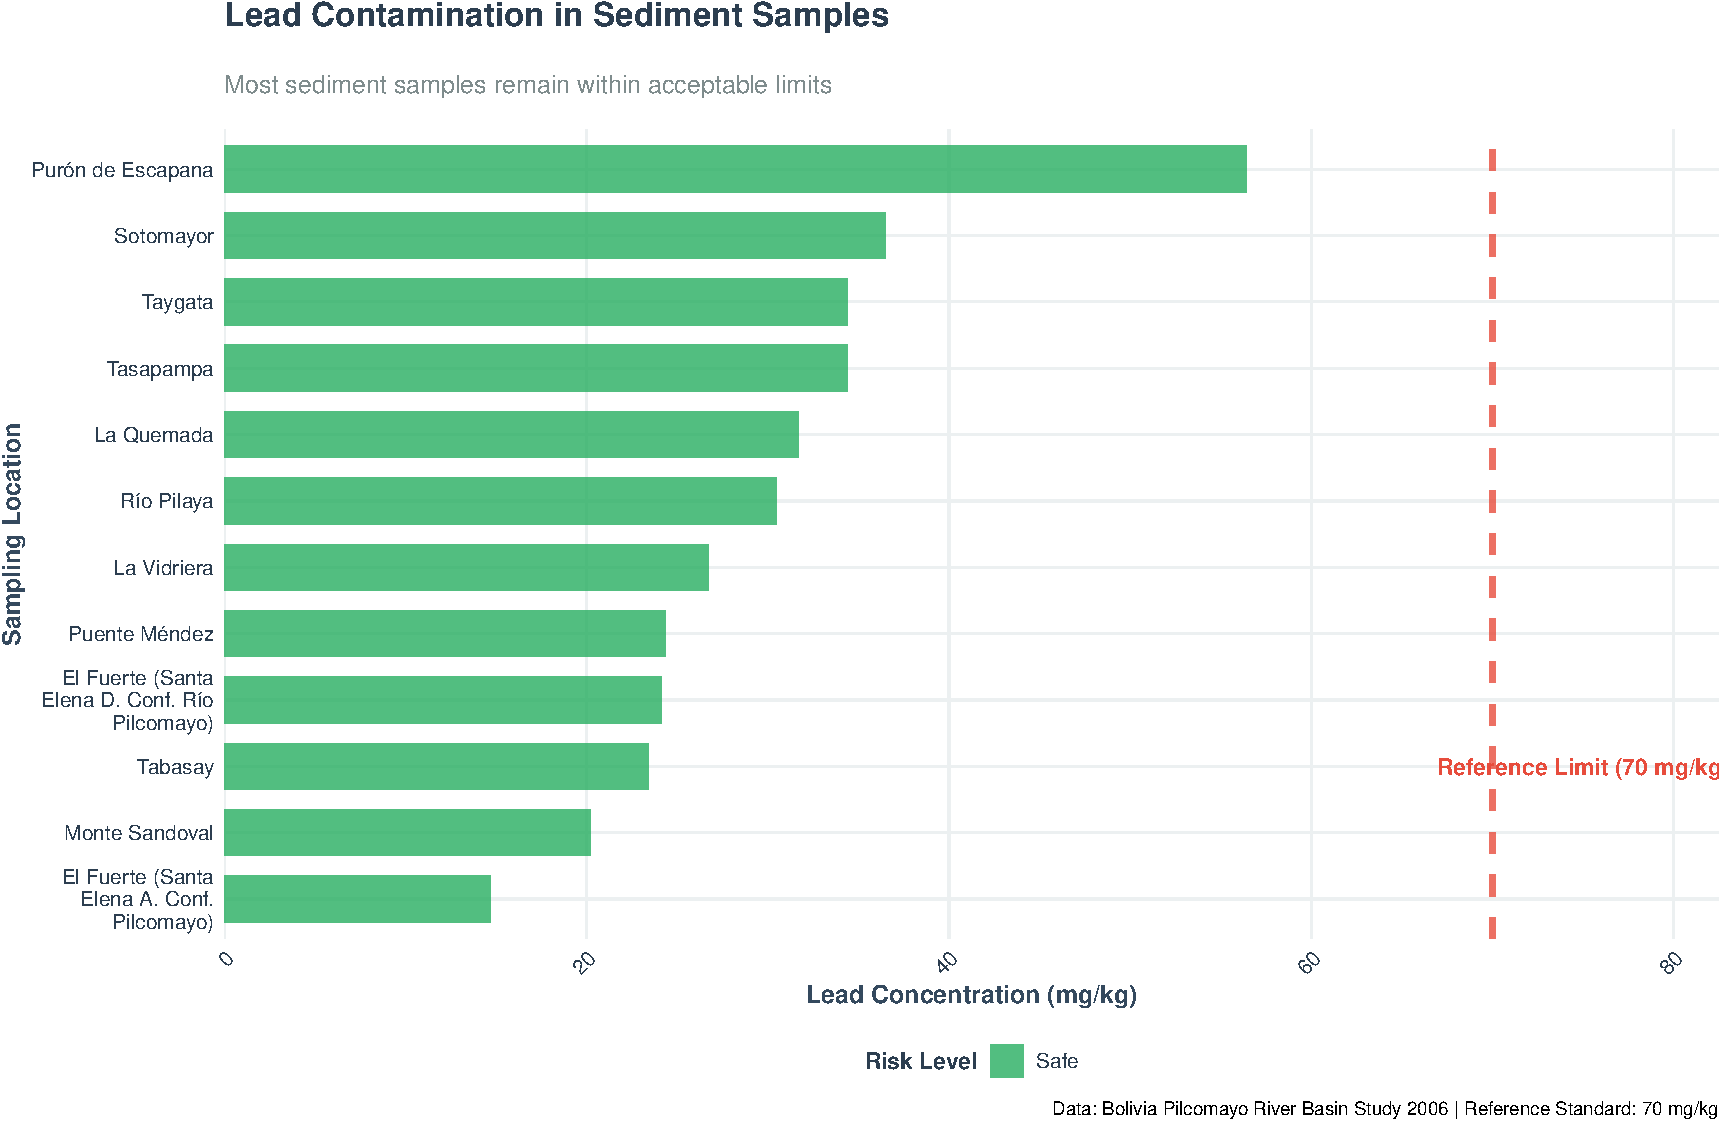
\includegraphics{WHO_standards_pdf_02_files/figure-latex/sediment-lead-1.pdf}

\begin{center}\rule{0.5\linewidth}{0.5pt}\end{center}

\section{Food Chain Contamination}\label{food-chain-contamination}

\begin{Shaded}
\begin{Highlighting}[]
\CommentTok{\# Load vegetation and fish data}
\NormalTok{veg }\OtherTok{\textless{}{-}} \FunctionTok{read\_csv}\NormalTok{(}\StringTok{"data/ITA\_veg\_2006.csv"}\NormalTok{)}
\NormalTok{fish }\OtherTok{\textless{}{-}} \FunctionTok{read\_csv}\NormalTok{(}\StringTok{"data/ITA\_fish\_2006.csv"}\NormalTok{)}

\CommentTok{\# Codex standard for lead in food}
\NormalTok{codex\_lead\_limit }\OtherTok{\textless{}{-}} \FloatTok{0.3}
\end{Highlighting}
\end{Shaded}

\subsection{Lead in Agricultural
Crops}\label{lead-in-agricultural-crops}

\begin{Shaded}
\begin{Highlighting}[]
\NormalTok{veg\_lead\_plot }\OtherTok{\textless{}{-}}\NormalTok{ veg }\SpecialCharTok{\%\textgreater{}\%}
  \FunctionTok{mutate}\NormalTok{(}
    \AttributeTok{exceeds\_limit =} \StringTok{\textasciigrave{}}\AttributeTok{Pb (mg/kg)}\StringTok{\textasciigrave{}} \SpecialCharTok{\textgreater{}}\NormalTok{ codex\_lead\_limit,}
    \AttributeTok{risk\_level =} \FunctionTok{case\_when}\NormalTok{(}
      \StringTok{\textasciigrave{}}\AttributeTok{Pb (mg/kg)}\StringTok{\textasciigrave{}} \SpecialCharTok{\textless{}=}\NormalTok{ codex\_lead\_limit }\SpecialCharTok{\textasciitilde{}} \StringTok{"Safe"}\NormalTok{,}
      \StringTok{\textasciigrave{}}\AttributeTok{Pb (mg/kg)}\StringTok{\textasciigrave{}} \SpecialCharTok{\textless{}=}\NormalTok{ codex\_lead\_limit }\SpecialCharTok{*} \DecValTok{3} \SpecialCharTok{\textasciitilde{}} \StringTok{"Moderate Risk"}\NormalTok{,}
      \StringTok{\textasciigrave{}}\AttributeTok{Pb (mg/kg)}\StringTok{\textasciigrave{}} \SpecialCharTok{\textless{}=}\NormalTok{ codex\_lead\_limit }\SpecialCharTok{*} \DecValTok{10} \SpecialCharTok{\textasciitilde{}} \StringTok{"High Risk"}\NormalTok{,}
      \ConstantTok{TRUE} \SpecialCharTok{\textasciitilde{}} \StringTok{"Critical Risk"}
\NormalTok{    )}
\NormalTok{  ) }\SpecialCharTok{\%\textgreater{}\%}
  \FunctionTok{ggplot}\NormalTok{(}\FunctionTok{aes}\NormalTok{(}\AttributeTok{x =} \FunctionTok{reorder}\NormalTok{(Crop, }\StringTok{\textasciigrave{}}\AttributeTok{Pb (mg/kg)}\StringTok{\textasciigrave{}}\NormalTok{), }\AttributeTok{y =} \StringTok{\textasciigrave{}}\AttributeTok{Pb (mg/kg)}\StringTok{\textasciigrave{}}\NormalTok{, }\AttributeTok{fill =}\NormalTok{ risk\_level)) }\SpecialCharTok{+}
  \FunctionTok{geom\_col}\NormalTok{(}\AttributeTok{alpha =} \FloatTok{0.8}\NormalTok{, }\AttributeTok{width =} \FloatTok{0.7}\NormalTok{) }\SpecialCharTok{+}
  \FunctionTok{geom\_hline}\NormalTok{(}
    \AttributeTok{yintercept =}\NormalTok{ codex\_lead\_limit, }
    \AttributeTok{color =}\NormalTok{ colors\_danger, }
    \AttributeTok{linetype =} \StringTok{"dashed"}\NormalTok{, }
    \AttributeTok{size =} \FloatTok{1.2}\NormalTok{,}
    \AttributeTok{alpha =} \FloatTok{0.8}
\NormalTok{  ) }\SpecialCharTok{+}
  \FunctionTok{annotate}\NormalTok{(}
    \StringTok{"text"}\NormalTok{,}
    \AttributeTok{x =} \DecValTok{3}\NormalTok{, }\AttributeTok{y =}\NormalTok{ codex\_lead\_limit }\SpecialCharTok{+} \DecValTok{2}\NormalTok{,}
    \AttributeTok{label =} \StringTok{"Codex Limit (0.3 mg/kg)"}\NormalTok{,}
    \AttributeTok{color =}\NormalTok{ colors\_danger,}
    \AttributeTok{size =} \DecValTok{4}\NormalTok{,}
    \AttributeTok{fontface =} \StringTok{"bold"}
\NormalTok{  ) }\SpecialCharTok{+}
  \FunctionTok{scale\_fill\_manual}\NormalTok{(}
    \AttributeTok{values =} \FunctionTok{c}\NormalTok{(}\StringTok{"Safe"} \OtherTok{=}\NormalTok{ colors\_safe, }
               \StringTok{"Moderate Risk"} \OtherTok{=}\NormalTok{ colors\_warning, }
               \StringTok{"High Risk"} \OtherTok{=} \StringTok{"\#e67e22"}\NormalTok{, }
               \StringTok{"Critical Risk"} \OtherTok{=}\NormalTok{ colors\_danger),}
    \AttributeTok{name =} \StringTok{"Risk Level"}
\NormalTok{  ) }\SpecialCharTok{+}
  \FunctionTok{scale\_y\_continuous}\NormalTok{(}
    \AttributeTok{labels =}\NormalTok{ scales}\SpecialCharTok{::}\FunctionTok{number\_format}\NormalTok{(}\AttributeTok{accuracy =} \FloatTok{0.1}\NormalTok{),}
    \AttributeTok{expand =} \FunctionTok{expansion}\NormalTok{(}\AttributeTok{mult =} \FunctionTok{c}\NormalTok{(}\DecValTok{0}\NormalTok{, }\FloatTok{0.1}\NormalTok{))}
\NormalTok{  ) }\SpecialCharTok{+}
  \FunctionTok{labs}\NormalTok{(}
    \AttributeTok{title =} \StringTok{"**Lead Contamination in Agricultural Crops**"}\NormalTok{,}
    \AttributeTok{subtitle =} \StringTok{"Most crops show severe contamination exceeding food safety standards"}\NormalTok{,}
    \AttributeTok{x =} \StringTok{"Crop Type"}\NormalTok{,}
    \AttributeTok{y =} \StringTok{"Lead Concentration (mg/kg)"}\NormalTok{,}
    \AttributeTok{caption =} \StringTok{"Data: Bolivia Pilcomayo River Basin Study 2006 | Codex Alimentarius Standard: 0.3 mg/kg"}
\NormalTok{  ) }\SpecialCharTok{+}
  \FunctionTok{theme\_enhanced}\NormalTok{() }\SpecialCharTok{+}
  \FunctionTok{coord\_flip}\NormalTok{()}

\NormalTok{veg\_lead\_plot}
\end{Highlighting}
\end{Shaded}

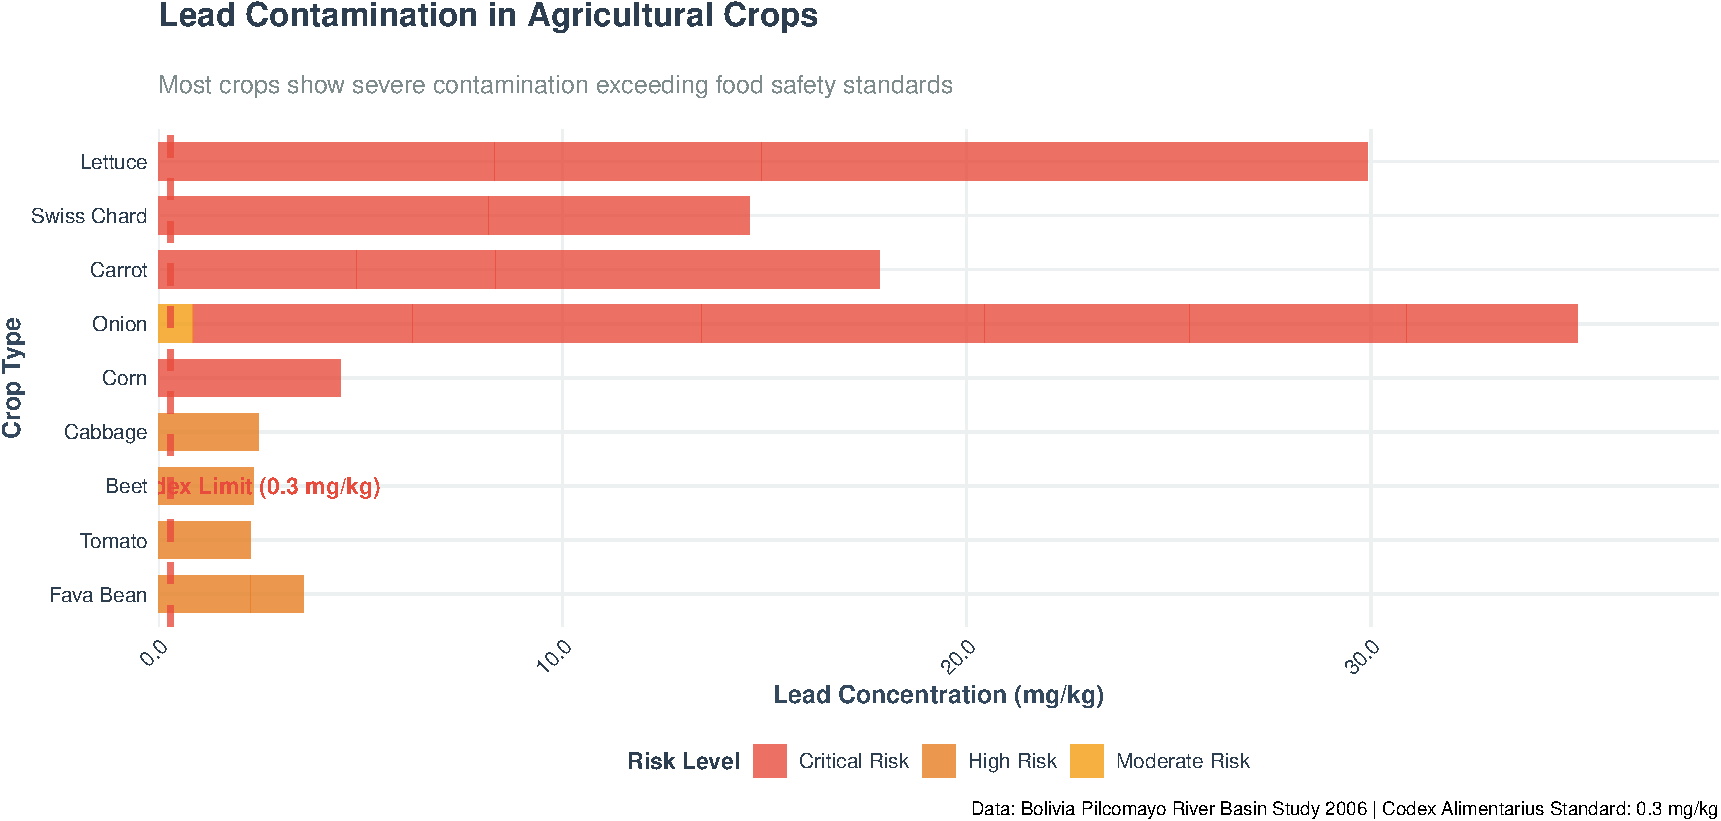
\includegraphics{WHO_standards_pdf_02_files/figure-latex/vegetation-lead-1.pdf}

\subsection{Lead in Fish and Aquatic
Life}\label{lead-in-fish-and-aquatic-life}

\begin{Shaded}
\begin{Highlighting}[]
\NormalTok{fish\_lead\_plot }\OtherTok{\textless{}{-}}\NormalTok{ fish }\SpecialCharTok{\%\textgreater{}\%}
  \FunctionTok{mutate}\NormalTok{(}
    \StringTok{\textasciigrave{}}\AttributeTok{Sample Type}\StringTok{\textasciigrave{}} \OtherTok{=} \FunctionTok{str\_replace\_all}\NormalTok{(}\StringTok{\textasciigrave{}}\AttributeTok{Sample Type}\StringTok{\textasciigrave{}}\NormalTok{, }\StringTok{" "}\NormalTok{, }\StringTok{"}\SpecialCharTok{\textbackslash{}n}\StringTok{"}\NormalTok{),}
    \AttributeTok{exceeds\_limit =} \StringTok{\textasciigrave{}}\AttributeTok{Pb (mg/kg)}\StringTok{\textasciigrave{}} \SpecialCharTok{\textgreater{}}\NormalTok{ codex\_lead\_limit,}
    \AttributeTok{risk\_level =} \FunctionTok{case\_when}\NormalTok{(}
      \StringTok{\textasciigrave{}}\AttributeTok{Pb (mg/kg)}\StringTok{\textasciigrave{}} \SpecialCharTok{\textless{}=}\NormalTok{ codex\_lead\_limit }\SpecialCharTok{\textasciitilde{}} \StringTok{"Safe"}\NormalTok{,}
      \StringTok{\textasciigrave{}}\AttributeTok{Pb (mg/kg)}\StringTok{\textasciigrave{}} \SpecialCharTok{\textless{}=}\NormalTok{ codex\_lead\_limit }\SpecialCharTok{*} \DecValTok{10} \SpecialCharTok{\textasciitilde{}} \StringTok{"High Risk"}\NormalTok{,}
      \ConstantTok{TRUE} \SpecialCharTok{\textasciitilde{}} \StringTok{"Critical Risk"}
\NormalTok{    )}
\NormalTok{  ) }\SpecialCharTok{\%\textgreater{}\%}
  \FunctionTok{ggplot}\NormalTok{(}\FunctionTok{aes}\NormalTok{(}\AttributeTok{x =} \FunctionTok{reorder}\NormalTok{(}\StringTok{\textasciigrave{}}\AttributeTok{Sample Type}\StringTok{\textasciigrave{}}\NormalTok{, }\StringTok{\textasciigrave{}}\AttributeTok{Pb (mg/kg)}\StringTok{\textasciigrave{}}\NormalTok{), }\AttributeTok{y =} \StringTok{\textasciigrave{}}\AttributeTok{Pb (mg/kg)}\StringTok{\textasciigrave{}}\NormalTok{, }\AttributeTok{fill =}\NormalTok{ risk\_level)) }\SpecialCharTok{+}
  \FunctionTok{geom\_col}\NormalTok{(}\AttributeTok{alpha =} \FloatTok{0.8}\NormalTok{, }\AttributeTok{width =} \FloatTok{0.6}\NormalTok{) }\SpecialCharTok{+}
  \FunctionTok{geom\_hline}\NormalTok{(}
    \AttributeTok{yintercept =}\NormalTok{ codex\_lead\_limit, }
    \AttributeTok{color =}\NormalTok{ colors\_danger, }
    \AttributeTok{linetype =} \StringTok{"dashed"}\NormalTok{, }
    \AttributeTok{size =} \FloatTok{1.2}\NormalTok{,}
    \AttributeTok{alpha =} \FloatTok{0.8}
\NormalTok{  ) }\SpecialCharTok{+}
  \FunctionTok{annotate}\NormalTok{(}
    \StringTok{"text"}\NormalTok{,}
    \AttributeTok{x =} \FloatTok{1.5}\NormalTok{, }\AttributeTok{y =}\NormalTok{ codex\_lead\_limit }\SpecialCharTok{+} \DecValTok{200}\NormalTok{,}
    \AttributeTok{label =} \StringTok{"Codex Limit}\SpecialCharTok{\textbackslash{}n}\StringTok{(0.3 mg/kg)"}\NormalTok{,}
    \AttributeTok{color =}\NormalTok{ colors\_danger,}
    \AttributeTok{size =} \DecValTok{4}\NormalTok{,}
    \AttributeTok{fontface =} \StringTok{"bold"}
\NormalTok{  ) }\SpecialCharTok{+}
  \FunctionTok{scale\_fill\_manual}\NormalTok{(}
    \AttributeTok{values =} \FunctionTok{c}\NormalTok{(}\StringTok{"Safe"} \OtherTok{=}\NormalTok{ colors\_safe, }
               \StringTok{"High Risk"} \OtherTok{=} \StringTok{"\#e67e22"}\NormalTok{, }
               \StringTok{"Critical Risk"} \OtherTok{=}\NormalTok{ colors\_danger),}
    \AttributeTok{name =} \StringTok{"Risk Level"}
\NormalTok{  ) }\SpecialCharTok{+}
  \FunctionTok{scale\_y\_continuous}\NormalTok{(}
    \AttributeTok{labels =}\NormalTok{ scales}\SpecialCharTok{::}\FunctionTok{comma\_format}\NormalTok{(),}
    \AttributeTok{expand =} \FunctionTok{expansion}\NormalTok{(}\AttributeTok{mult =} \FunctionTok{c}\NormalTok{(}\DecValTok{0}\NormalTok{, }\FloatTok{0.1}\NormalTok{))}
\NormalTok{  ) }\SpecialCharTok{+}
  \FunctionTok{labs}\NormalTok{(}
    \AttributeTok{title =} \StringTok{"**Lead Contamination in Fish and Aquatic Life**"}\NormalTok{,}
    \AttributeTok{subtitle =} \StringTok{"Critical contamination levels in fish heads and small fish samples"}\NormalTok{,}
    \AttributeTok{x =} \StringTok{"Sample Type"}\NormalTok{,}
    \AttributeTok{y =} \StringTok{"Lead Concentration (mg/kg)"}\NormalTok{,}
    \AttributeTok{caption =} \StringTok{"Data: Bolivia Pilcomayo River Basin Study 2006 | Codex Alimentarius Standard: 0.3 mg/kg"}
\NormalTok{  ) }\SpecialCharTok{+}
  \FunctionTok{theme\_enhanced}\NormalTok{()}

\NormalTok{fish\_lead\_plot}
\end{Highlighting}
\end{Shaded}

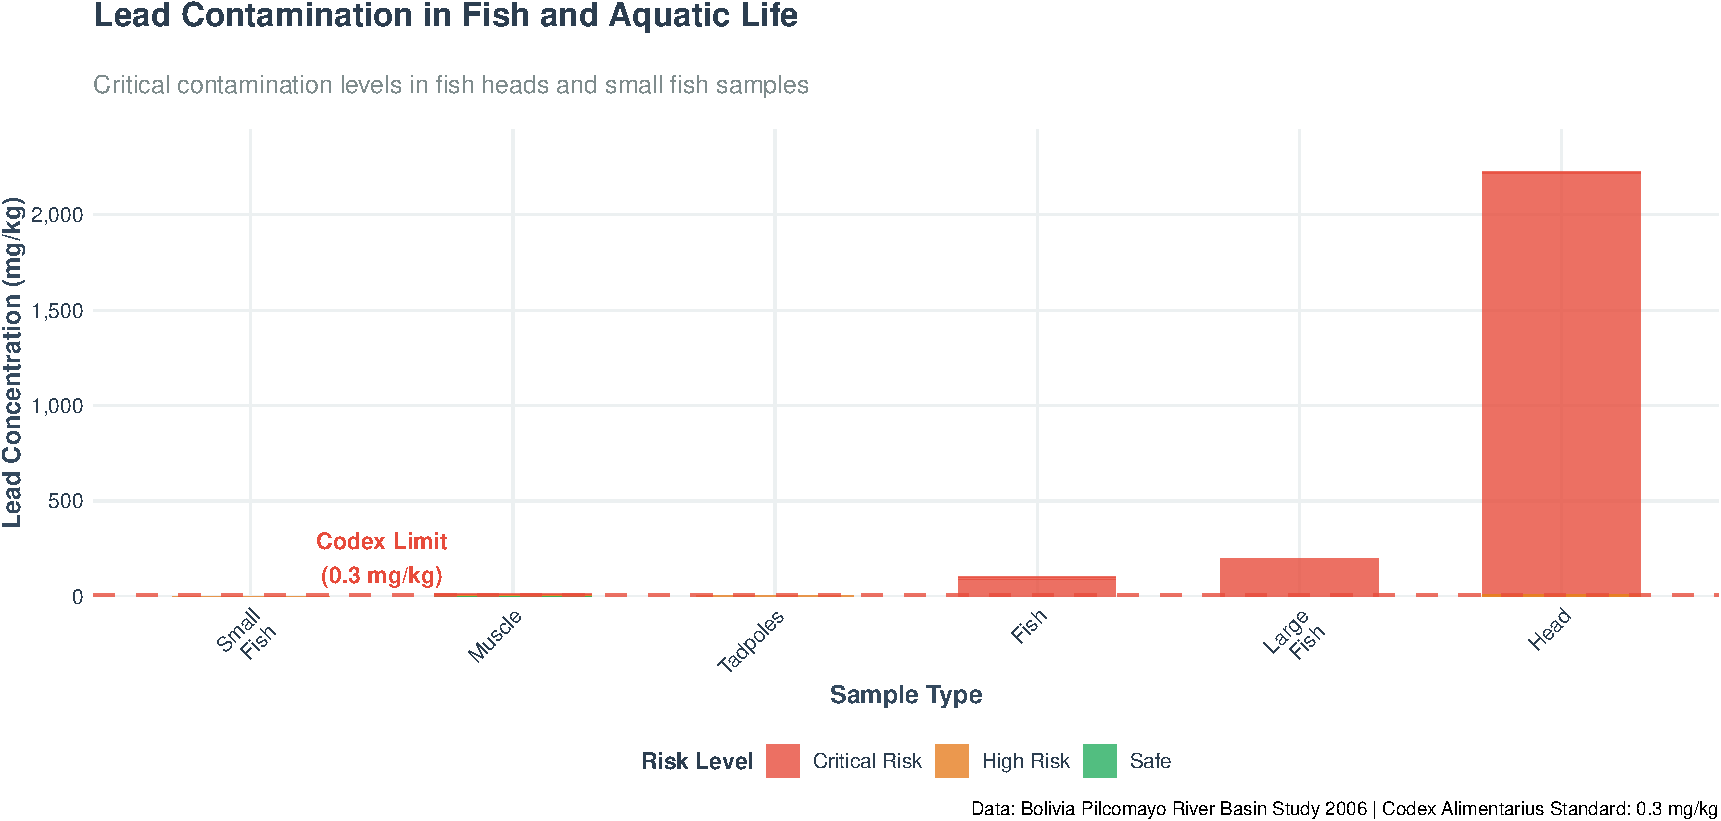
\includegraphics{WHO_standards_pdf_02_files/figure-latex/fish-lead-1.pdf}

\begin{center}\rule{0.5\linewidth}{0.5pt}\end{center}

\section{Human and Animal Health
Impact}\label{human-and-animal-health-impact}

\begin{Shaded}
\begin{Highlighting}[]
\CommentTok{\# Load human and animal data}
\NormalTok{human }\OtherTok{\textless{}{-}} \FunctionTok{read\_csv}\NormalTok{(}\StringTok{"data/ITA\_human\_2006.csv"}\NormalTok{)}
\NormalTok{animal }\OtherTok{\textless{}{-}} \FunctionTok{read\_csv}\NormalTok{(}\StringTok{"data/ITA\_animal\_2006.csv"}\NormalTok{)}

\CommentTok{\# CDC reference value for lead in children\textquotesingle{}s blood}
\NormalTok{cdc\_lead\_limit }\OtherTok{\textless{}{-}} \DecValTok{5}
\CommentTok{\# Veterinary threshold for lead in animals}
\NormalTok{vet\_lead\_limit }\OtherTok{\textless{}{-}} \FloatTok{0.3}
\end{Highlighting}
\end{Shaded}

\subsection{Lead in Children's Blood}\label{lead-in-childrens-blood}

\begin{Shaded}
\begin{Highlighting}[]
\CommentTok{\# Aggregate data by location and use mean values for children}
\NormalTok{human\_summary }\OtherTok{\textless{}{-}}\NormalTok{ human }\SpecialCharTok{\%\textgreater{}\%}
  \FunctionTok{group\_by}\NormalTok{(Location) }\SpecialCharTok{\%\textgreater{}\%}
  \FunctionTok{summarise}\NormalTok{(}
    \AttributeTok{mean\_pb\_children =} \FunctionTok{mean}\NormalTok{(}\StringTok{\textasciigrave{}}\AttributeTok{Mean Pb [µg/dl] Children}\StringTok{\textasciigrave{}}\NormalTok{, }\AttributeTok{na.rm =} \ConstantTok{TRUE}\NormalTok{),}
    \AttributeTok{.groups =} \StringTok{\textquotesingle{}drop\textquotesingle{}}
\NormalTok{  ) }\SpecialCharTok{\%\textgreater{}\%}
  \FunctionTok{filter}\NormalTok{(}\SpecialCharTok{!}\FunctionTok{is.na}\NormalTok{(mean\_pb\_children)) }\SpecialCharTok{\%\textgreater{}\%}
  \FunctionTok{mutate}\NormalTok{(}
    \AttributeTok{Location =} \FunctionTok{str\_wrap}\NormalTok{(Location, }\DecValTok{15}\NormalTok{),}
    \AttributeTok{exceeds\_limit =}\NormalTok{ mean\_pb\_children }\SpecialCharTok{\textgreater{}}\NormalTok{ cdc\_lead\_limit,}
    \AttributeTok{risk\_level =} \FunctionTok{case\_when}\NormalTok{(}
\NormalTok{      mean\_pb\_children }\SpecialCharTok{\textless{}=}\NormalTok{ cdc\_lead\_limit }\SpecialCharTok{\textasciitilde{}} \StringTok{"Safe"}\NormalTok{,}
\NormalTok{      mean\_pb\_children }\SpecialCharTok{\textless{}=}\NormalTok{ cdc\_lead\_limit }\SpecialCharTok{*} \DecValTok{2} \SpecialCharTok{\textasciitilde{}} \StringTok{"Moderate Risk"}\NormalTok{,}
\NormalTok{      mean\_pb\_children }\SpecialCharTok{\textless{}=}\NormalTok{ cdc\_lead\_limit }\SpecialCharTok{*} \DecValTok{3} \SpecialCharTok{\textasciitilde{}} \StringTok{"High Risk"}\NormalTok{,}
      \ConstantTok{TRUE} \SpecialCharTok{\textasciitilde{}} \StringTok{"Critical Risk"}
\NormalTok{    )}
\NormalTok{  )}

\NormalTok{human\_lead\_plot }\OtherTok{\textless{}{-}}\NormalTok{ human\_summary }\SpecialCharTok{\%\textgreater{}\%}
  \FunctionTok{ggplot}\NormalTok{(}\FunctionTok{aes}\NormalTok{(}\AttributeTok{x =} \FunctionTok{reorder}\NormalTok{(Location, mean\_pb\_children), }\AttributeTok{y =}\NormalTok{ mean\_pb\_children, }\AttributeTok{fill =}\NormalTok{ risk\_level)) }\SpecialCharTok{+}
  \FunctionTok{geom\_col}\NormalTok{(}\AttributeTok{alpha =} \FloatTok{0.8}\NormalTok{, }\AttributeTok{width =} \FloatTok{0.7}\NormalTok{) }\SpecialCharTok{+}
  \FunctionTok{geom\_hline}\NormalTok{(}
    \AttributeTok{yintercept =}\NormalTok{ cdc\_lead\_limit, }
    \AttributeTok{color =}\NormalTok{ colors\_danger, }
    \AttributeTok{linetype =} \StringTok{"dashed"}\NormalTok{, }
    \AttributeTok{size =} \FloatTok{1.2}\NormalTok{,}
    \AttributeTok{alpha =} \FloatTok{0.8}
\NormalTok{  ) }\SpecialCharTok{+}
  \FunctionTok{annotate}\NormalTok{(}
    \StringTok{"text"}\NormalTok{,}
    \AttributeTok{x =} \DecValTok{3}\NormalTok{, }\AttributeTok{y =}\NormalTok{ cdc\_lead\_limit }\SpecialCharTok{+} \DecValTok{1}\NormalTok{,}
    \AttributeTok{label =} \StringTok{"CDC Reference (5 μg/dL)"}\NormalTok{,}
    \AttributeTok{color =}\NormalTok{ colors\_danger,}
    \AttributeTok{size =} \DecValTok{4}\NormalTok{,}
    \AttributeTok{fontface =} \StringTok{"bold"}
\NormalTok{  ) }\SpecialCharTok{+}
  \FunctionTok{scale\_fill\_manual}\NormalTok{(}
    \AttributeTok{values =} \FunctionTok{c}\NormalTok{(}\StringTok{"Safe"} \OtherTok{=}\NormalTok{ colors\_safe, }
               \StringTok{"Moderate Risk"} \OtherTok{=}\NormalTok{ colors\_warning, }
               \StringTok{"High Risk"} \OtherTok{=} \StringTok{"\#e67e22"}\NormalTok{, }
               \StringTok{"Critical Risk"} \OtherTok{=}\NormalTok{ colors\_danger),}
    \AttributeTok{name =} \StringTok{"Risk Level"}
\NormalTok{  ) }\SpecialCharTok{+}
  \FunctionTok{scale\_y\_continuous}\NormalTok{(}
    \AttributeTok{labels =}\NormalTok{ scales}\SpecialCharTok{::}\FunctionTok{number\_format}\NormalTok{(}\AttributeTok{accuracy =} \FloatTok{0.1}\NormalTok{),}
    \AttributeTok{expand =} \FunctionTok{expansion}\NormalTok{(}\AttributeTok{mult =} \FunctionTok{c}\NormalTok{(}\DecValTok{0}\NormalTok{, }\FloatTok{0.1}\NormalTok{))}
\NormalTok{  ) }\SpecialCharTok{+}
  \FunctionTok{labs}\NormalTok{(}
    \AttributeTok{title =} \StringTok{"**Lead Exposure in Children\textquotesingle{}s Blood (Community Averages)**"}\NormalTok{,}
    \AttributeTok{subtitle =} \StringTok{"Several communities show elevated lead levels exceeding CDC reference values"}\NormalTok{,}
    \AttributeTok{x =} \StringTok{"Community Location"}\NormalTok{,}
    \AttributeTok{y =} \StringTok{"Mean Blood Lead Level (µg/dL)"}\NormalTok{,}
    \AttributeTok{caption =} \StringTok{"Data: Bolivia Pilcomayo River Basin Study 2006 | CDC Reference Value: 5 µg/dL"}
\NormalTok{  ) }\SpecialCharTok{+}
  \FunctionTok{theme\_enhanced}\NormalTok{() }\SpecialCharTok{+}
  \FunctionTok{coord\_flip}\NormalTok{()}

\NormalTok{human\_lead\_plot}
\end{Highlighting}
\end{Shaded}

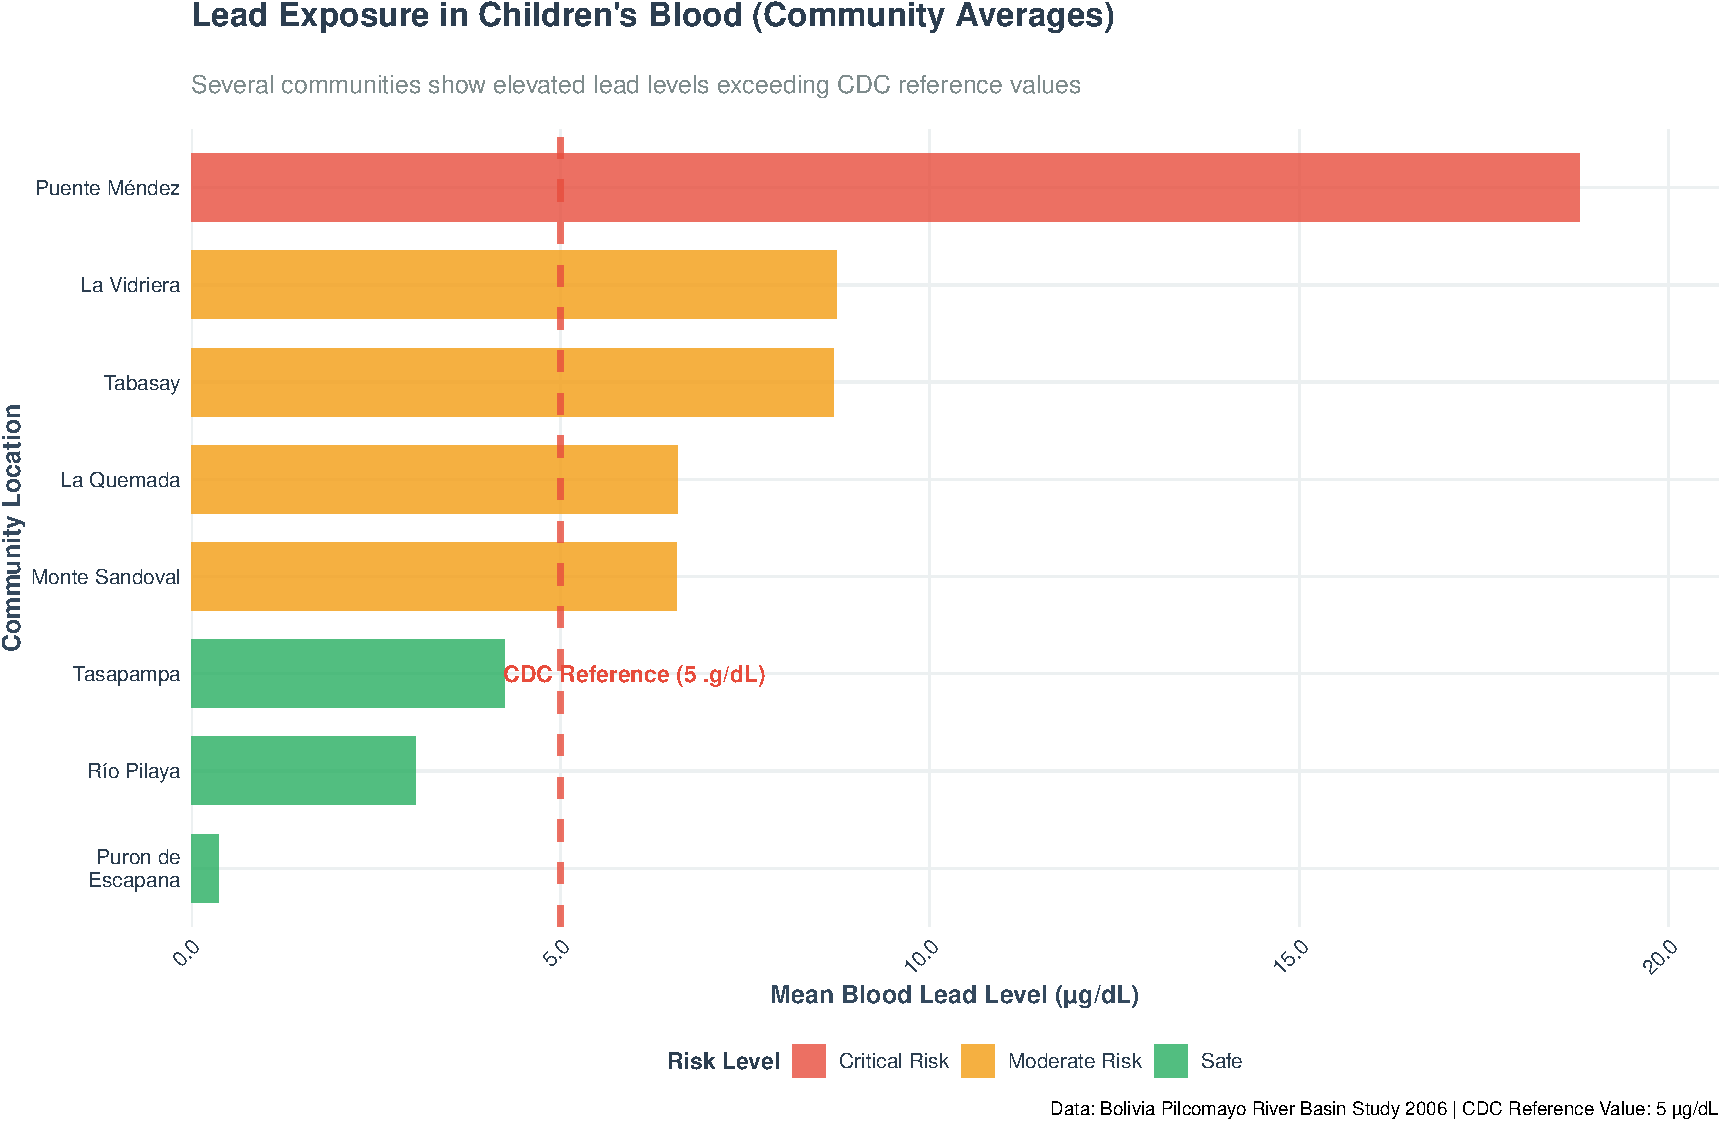
\includegraphics{WHO_standards_pdf_02_files/figure-latex/human-lead-1.pdf}

\subsection{Lead in Livestock Blood}\label{lead-in-livestock-blood}

\begin{Shaded}
\begin{Highlighting}[]
\NormalTok{animal\_lead\_plot }\OtherTok{\textless{}{-}}\NormalTok{ animal }\SpecialCharTok{\%\textgreater{}\%}
  \FunctionTok{mutate}\NormalTok{(}
    \AttributeTok{exceeds\_limit =} \StringTok{\textasciigrave{}}\AttributeTok{Pb (mg/dL)}\StringTok{\textasciigrave{}} \SpecialCharTok{\textgreater{}}\NormalTok{ vet\_lead\_limit,}
    \AttributeTok{risk\_level =} \FunctionTok{case\_when}\NormalTok{(}
      \StringTok{\textasciigrave{}}\AttributeTok{Pb (mg/dL)}\StringTok{\textasciigrave{}} \SpecialCharTok{\textless{}=}\NormalTok{ vet\_lead\_limit }\SpecialCharTok{\textasciitilde{}} \StringTok{"Safe"}\NormalTok{,}
      \StringTok{\textasciigrave{}}\AttributeTok{Pb (mg/dL)}\StringTok{\textasciigrave{}} \SpecialCharTok{\textless{}=}\NormalTok{ vet\_lead\_limit }\SpecialCharTok{*} \DecValTok{5} \SpecialCharTok{\textasciitilde{}} \StringTok{"Moderate Risk"}\NormalTok{,}
      \StringTok{\textasciigrave{}}\AttributeTok{Pb (mg/dL)}\StringTok{\textasciigrave{}} \SpecialCharTok{\textless{}=}\NormalTok{ vet\_lead\_limit }\SpecialCharTok{*} \DecValTok{20} \SpecialCharTok{\textasciitilde{}} \StringTok{"High Risk"}\NormalTok{,}
      \ConstantTok{TRUE} \SpecialCharTok{\textasciitilde{}} \StringTok{"Critical Risk"}
\NormalTok{    )}
\NormalTok{  ) }\SpecialCharTok{\%\textgreater{}\%}
  \FunctionTok{ggplot}\NormalTok{(}\FunctionTok{aes}\NormalTok{(}\AttributeTok{x =} \FunctionTok{reorder}\NormalTok{(Animal, }\StringTok{\textasciigrave{}}\AttributeTok{Pb (mg/dL)}\StringTok{\textasciigrave{}}\NormalTok{), }\AttributeTok{y =} \StringTok{\textasciigrave{}}\AttributeTok{Pb (mg/dL)}\StringTok{\textasciigrave{}}\NormalTok{, }\AttributeTok{fill =}\NormalTok{ risk\_level)) }\SpecialCharTok{+}
  \FunctionTok{geom\_col}\NormalTok{(}\AttributeTok{alpha =} \FloatTok{0.8}\NormalTok{, }\AttributeTok{width =} \FloatTok{0.7}\NormalTok{) }\SpecialCharTok{+}
  \FunctionTok{geom\_hline}\NormalTok{(}
    \AttributeTok{yintercept =}\NormalTok{ vet\_lead\_limit, }
    \AttributeTok{color =}\NormalTok{ colors\_danger, }
    \AttributeTok{linetype =} \StringTok{"dashed"}\NormalTok{, }
    \AttributeTok{size =} \FloatTok{1.2}\NormalTok{,}
    \AttributeTok{alpha =} \FloatTok{0.8}
\NormalTok{  ) }\SpecialCharTok{+}
  \FunctionTok{annotate}\NormalTok{(}
    \StringTok{"text"}\NormalTok{,}
    \AttributeTok{x =} \DecValTok{3}\NormalTok{, }\AttributeTok{y =}\NormalTok{ vet\_lead\_limit }\SpecialCharTok{+} \DecValTok{5}\NormalTok{,}
    \AttributeTok{label =} \StringTok{"Veterinary Threshold}\SpecialCharTok{\textbackslash{}n}\StringTok{(\textasciitilde{}0.3 mg/dL)"}\NormalTok{,}
    \AttributeTok{color =}\NormalTok{ colors\_danger,}
    \AttributeTok{size =} \DecValTok{4}\NormalTok{,}
    \AttributeTok{fontface =} \StringTok{"bold"}
\NormalTok{  ) }\SpecialCharTok{+}
  \FunctionTok{scale\_fill\_manual}\NormalTok{(}
    \AttributeTok{values =} \FunctionTok{c}\NormalTok{(}\StringTok{"Safe"} \OtherTok{=}\NormalTok{ colors\_safe, }
               \StringTok{"Moderate Risk"} \OtherTok{=}\NormalTok{ colors\_warning, }
               \StringTok{"High Risk"} \OtherTok{=} \StringTok{"\#e67e22"}\NormalTok{, }
               \StringTok{"Critical Risk"} \OtherTok{=}\NormalTok{ colors\_danger),}
    \AttributeTok{name =} \StringTok{"Risk Level"}
\NormalTok{  ) }\SpecialCharTok{+}
  \FunctionTok{scale\_y\_continuous}\NormalTok{(}
    \AttributeTok{labels =}\NormalTok{ scales}\SpecialCharTok{::}\FunctionTok{number\_format}\NormalTok{(}\AttributeTok{accuracy =} \FloatTok{0.1}\NormalTok{),}
    \AttributeTok{expand =} \FunctionTok{expansion}\NormalTok{(}\AttributeTok{mult =} \FunctionTok{c}\NormalTok{(}\DecValTok{0}\NormalTok{, }\FloatTok{0.1}\NormalTok{))}
\NormalTok{  ) }\SpecialCharTok{+}
  \FunctionTok{labs}\NormalTok{(}
    \AttributeTok{title =} \StringTok{"**Lead Exposure in Livestock Blood**"}\NormalTok{,}
    \AttributeTok{subtitle =} \StringTok{"All livestock species show severe lead poisoning levels"}\NormalTok{,}
    \AttributeTok{x =} \StringTok{"Animal Type"}\NormalTok{,}
    \AttributeTok{y =} \StringTok{"Blood Lead Level (mg/dL)"}\NormalTok{,}
    \AttributeTok{caption =} \StringTok{"Data: Bolivia Pilcomayo River Basin Study 2006 | Veterinary Threshold: \textasciitilde{}0.3 mg/dL"}
\NormalTok{  ) }\SpecialCharTok{+}
  \FunctionTok{theme\_enhanced}\NormalTok{()}

\NormalTok{animal\_lead\_plot}
\end{Highlighting}
\end{Shaded}

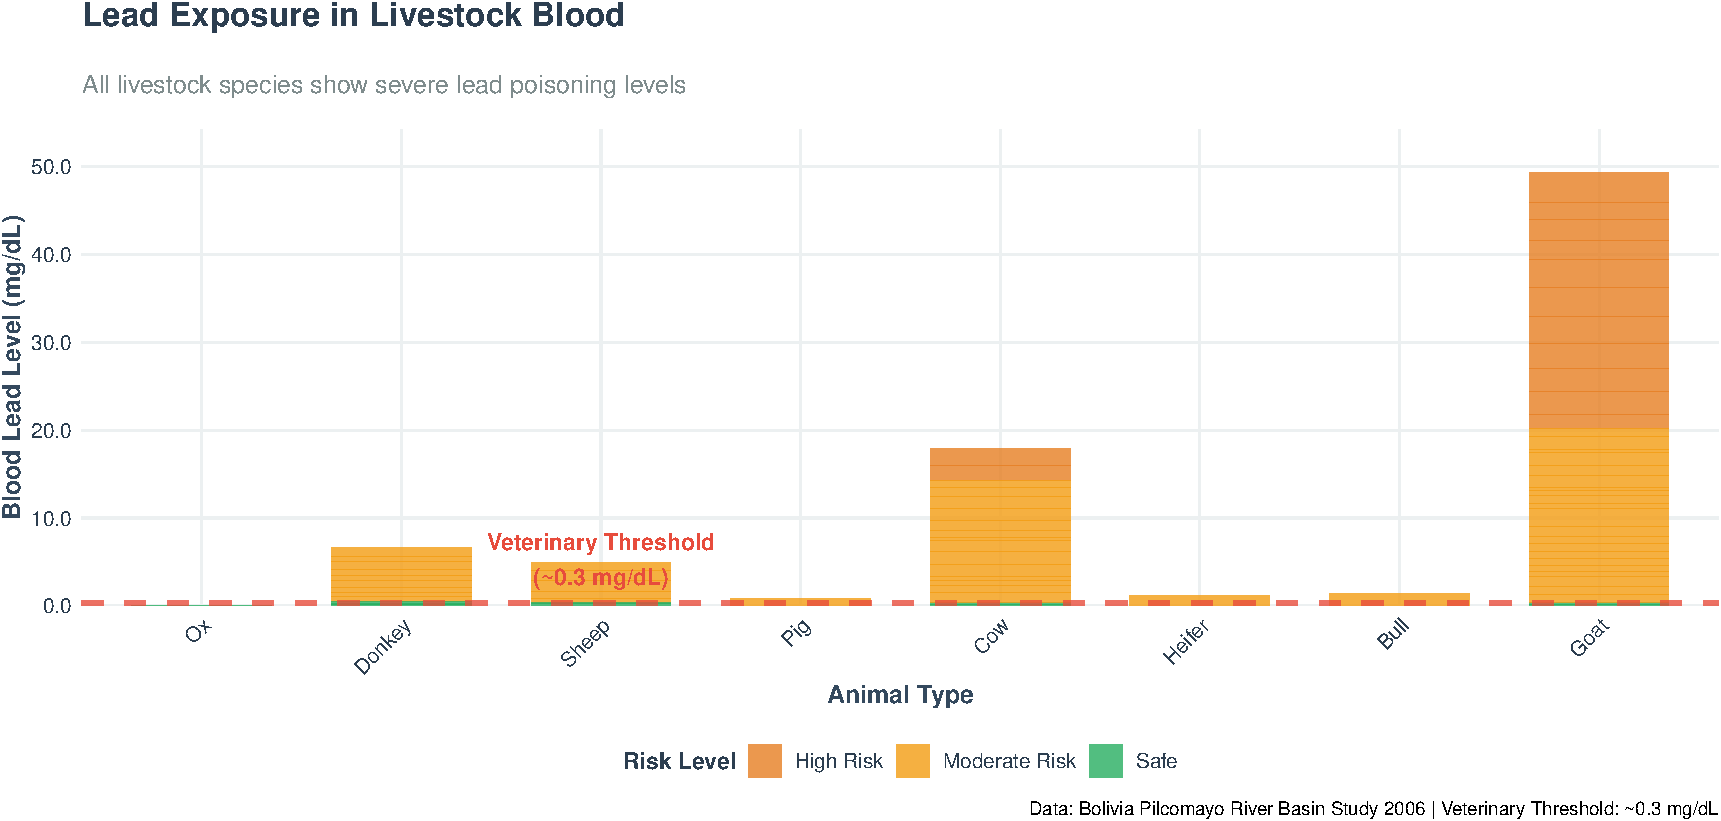
\includegraphics{WHO_standards_pdf_02_files/figure-latex/animal-lead-1.pdf}

\begin{center}\rule{0.5\linewidth}{0.5pt}\end{center}

\section{Summary and Conclusions}\label{summary-and-conclusions}

\subsection{Key Findings}\label{key-findings}

This comprehensive analysis of heavy metal contamination in the
Pilcomayo River basin reveals \textbf{critical environmental and public
health concerns}:

\subsubsection{\texorpdfstring{🚨 \textbf{Critical Contamination
Areas}}{🚨 Critical Contamination Areas}}\label{critical-contamination-areas}

\begin{itemize}
\tightlist
\item
  \textbf{Water Sources}: Multiple locations exceed WHO lead standards
  by 10-80 times
\item
  \textbf{Agricultural Crops}: Most crops show lead levels 10-100 times
  above Codex food safety limits\\
\item
  \textbf{Fish and Aquatic Life}: Critical contamination in fish heads
  (\textgreater6000x safe levels)
\item
  \textbf{Human Health}: Children in several communities exceed CDC
  reference values
\item
  \textbf{Livestock}: All animal species show severe lead poisoning
  levels
\end{itemize}

\subsubsection{\texorpdfstring{📊 \textbf{Contamination Severity
Rankings}}{📊 Contamination Severity Rankings}}\label{contamination-severity-rankings}

\begin{enumerate}
\def\labelenumi{\arabic{enumi}.}
\tightlist
\item
  \textbf{Fish/Aquatic samples} - Most severely contaminated
\item
  \textbf{Soil samples} - High contamination in multiple locations
\item
  \textbf{Agricultural crops} - Widespread food safety concerns
\item
  \textbf{Livestock blood} - Severe poisoning across all species
\item
  \textbf{Children's blood} - Elevated levels in multiple communities
\item
  \textbf{Water sources} - Several locations exceed safe drinking limits
\end{enumerate}

\subsubsection{\texorpdfstring{🔬 \textbf{Environmental
Impact}}{🔬 Environmental Impact}}\label{environmental-impact}

The contamination appears to follow the water-soil-plant-animal-human
pathway, indicating \textbf{systemic environmental pollution} that
requires immediate intervention.

\subsection{Recommendations}\label{recommendations}

\begin{enumerate}
\def\labelenumi{\arabic{enumi}.}
\tightlist
\item
  \textbf{Immediate Actions}: Restrict consumption of locally grown
  crops and fish
\item
  \textbf{Water Treatment}: Implement water purification systems for
  affected communities\\
\item
  \textbf{Soil Remediation}: Begin soil treatment programs in highly
  contaminated areas
\item
  \textbf{Health Monitoring}: Establish regular blood lead monitoring
  for children and pregnant women
\item
  \textbf{Source Control}: Identify and eliminate lead contamination
  sources
\item
  \textbf{Long-term Monitoring}: Implement continuous environmental
  monitoring program
\end{enumerate}

\begin{center}\rule{0.5\linewidth}{0.5pt}\end{center}

\emph{This analysis is based on 2006 data from the Bolivia Pilcomayo
River Basin Study. Current conditions may differ and require updated
assessment.}

\end{document}
